%%%%%%%%%%%%%%%%%%%%%%%%%%%%%%%%%%%%%%%%%%%%%%%%%%%%
% U T F P R  /  C  O R N � L I O   P R O C � P I O %
%%%%%%%%%%%%%%%%%%%%%%%%%%%%%%%%%%%%%%%%%%%%%%%%%%%%
%  MODELO PARA PROPOSTA / TRABALHO DE DIPLOMA��O   %
%                                                  %
% E Q U I P E :                                    %
%                                                  %
% DIOGO CEZAR TEIXEIRA BATISTA                     %
% <xgordo@gmail.com>                               %
%                                                  %
% RAFAEL AUGUSTO AMBROSIO ROSA                     %
% <rafarafarosa@hotmail.com>                       %
%                                                  %
% In�cio : Agosto/2006                             %
%%%%%%%%%%%%%%%%%%%%%%%%%%%%%%%%%%%%%%%%%%%%%%%%%%%%

\documentclass[a4paper,noheader,indentfirst,pnumplain,times,tocpage=plain,estilo=UTFPR,abnt-url-package=url]{abnt}

\usepackage[brazil]{babel}
\usepackage[latin1]{inputenc}
\usepackage[T1]{fontenc}
\usepackage{sty/tabela-simbolos}
\usepackage{sty/makeglo}
\usepackage{sty/utfPR}
\usepackage{sty/listings}
\usepackage{sty/listequations}
\usepackage{graphicx,url}
\usepackage{fancyhdr}
\usepackage[lmargin=3cm,tmargin=3cm,rmargin=1.5cm,bmargin=1.5cm]{geometry}
\usepackage[pdftex]{lscape}
\usepackage{longtable}
\usepackage[alf,abnt-and-type=e,abnt-etal-cite=2, bibjustif]{abntcite}
\usepackage{amsmath}
\usepackage{float}
\usepackage{qtree}
\usepackage{supertabular}
\usepackage{color}

\UTFPRconfigs

\UTFPRmakeglossario

%%%%%%%%%%%%%%%%%%%%%%%%%%%%%%%%%%%%%%%%%%%%%%%%%%%%
% C O N F I G U R A � � E S  D O S   C � D I G O S %
%%%%%%%%%%%%%%%%%%%%%%%%%%%%%%%%%%%%%%%%%%%%%%%%%%%%

\lstset{numbers=left, stepnumber=1, firstnumber=1,
numberstyle=\tiny, extendedchars=true, breaklines=true,frame=tb,
basicstyle=\scriptsize, stringstyle=\scriptsize,
showstringspaces=false}

\renewcommand{\lstlistingname}{C�digo}
\renewcommand{\lstlistlistingname}{LISTA DE C�DIGOS}

\begin{document}

    %%%%%%%%%%%%%%%%%%%%%%%%%%%%%%%%%%%%%%%%%%%%%%%
    % E L E M E N T O S  P R E - T E X  T U A I S %
    %%%%%%%%%%%%%%%%%%%%%%%%%%%%%%%%%%%%%%%%%%%%%%%

    \UTFPRnumRomanos

    \UTFPRdedicatoria{
    Aos meus pais,      \\
A minha irm�,       \\
A minha orientadora.

    }

    \UTFPRagradecimentos{
    Agrade�o a Deus pela sa�de que me foi concedida para realizar esse
trabalho.

Agrade�o aos meus familiares em especial o mais pr�ximos, minha m�e
querida Izabel Cristina Jos� Teixeira Batista, meu pai M�rio Sergio
Batista e a minha irm� Mayra Cristina Teixeira Batista, que me
apoiaram e me confortaram nos �rduos momentos que enfrentei.
Agrade�o a eles tamb�m pela oportunidade da plena dedica��o aos
estudos, ajudando com meus custos at� conclus�o do curso. Ainda na
fam�lia agrade�o � meu primo jornalista Roberto Cezar Teixeira
Pereira, que muito me auxiliou e incentivou na elabora��o da
monografia. E por fim a todos meus familiares, que sempre se
interessavam em saber como andava a universidade.

Agrade�o a meus queridos amigos de estudos, o famoso grupo
"Kakitus", formado por: Marlos Henrique dos Santos (Fofys), Rafael
Augusto Ambr�sio Rosa (Rafinha, Rafiusk, Rafa), Fernando Jos�
Parissenti, esse teve que me ag�entar, e muito! mais conhecido como
Z�, Fernando Akimoto Tadashi ou s� Tadashi, e ao Rafael Feresini ou
Xandy mesmo. Agrade�o tamb�m outros amigos da faculdade que ajudaram
nessa caminhada: Henrique Shishido, Igor, Mario, Paulo, Aninha e J�,
e ainda amigos �ntimos que sempre me apoiaram e estiveram do meu
lado: Mari (namorada do Leo), Leonardo, Luiz Eduardo, Ferdinando,
J�nior, Guliver, Galileu, Yoda (Por n�o me morder), Corisco, Mayra,
Roger, Bacalhau. Pessoal, n�o h� palavras para expressar os
maravilhosos momentos de descontra��o e sabedoria que
compartilhamos, por tudo isso s� quero dizer: OBRIGADO!

Obrigado ao pessoal das minhas bandas que puderam compreender
algumas aus�ncias nos ensaios para a elabora��o desse trabalho.

Em especial, gostaria de agradecer aos professores: Guilherme,
Thesko, Ant�nio e Gabriel que puderam compartilhar seus
conhecimentos da melhor maneira poss�vel, atrav�s da amizade.

Ainda gostaria de agradecer a uma pessoa especial, que colaborou de
forma direta para que esse projeto pudesse ser conclu�do com exito,
uma pessoa que mais que orientadora ou instrutora, se tornou uma
querida amiga e sempre poder� contar comigo. Professora L�gia, para
t�, o meu humilde MUITO OBRIGADO.

Enfim obrigado a todos que de forma direta ou indireta colaboraram
de alguma forma para o sucesso deste trabalho e para o meu sucesso.

    }

    \UTFPRepigrafe{Escolha um trabalho que voc� ame e n�o ter�s que trabalhar um �nico dia em sua vida}{Conf�cio}

    \UTFPRresumo[Hiperm�dia Adaptativa, Orienta��o, Otimiza��o por Col�nia de Formigas, Navega��o Colaborativa]{
    Experimentos cient�ficos produzem grande quantidade de informa��es que necessitam de processamento para uma posterior an�lise. Um cientista, que n�o � da �rea da computa��o, nem sempre possui as habilidades para desenvolver seu pr�prio ambiente de testes. Por isso a utiliza��o de executores de fluxos de trabalhos cient�ficos v�m sido largamente estudada. Uma das principais vantagens de se utilizar um processador de fluxo de trabalho cient�fico � a transpar�ncia oferecida para o cientista em rela��o a maneira com que os experimentos ser�o organizados, distribu�dos e processados. Este trabalho prop�e um modelo para cria��o de um ambiente que seja capaz de processar esses fluxos de trabalho. A �nfase est� em um escalonamento inteligente que utiliza t�cnicas para resolu��o de problemas de planejamento da �rea de intelig�ncia artificial.
    }

    \UTFPRabstract[Adaptative Hypermedia, Orientation, Ant Colony Optimization,Collaborative Navigation.]{
    Scientific experiments produce a large amount of information that require processing for further analysis. A scientist, that not work in computing area, does not always have the skills to develop their own test environment. Therefore the usage of executors of scientific workflows have been widely studied. The main advantage in use a workflow scientific processor is the transparency offered for the scientist regarding the manner in which the experiments will be organized, distributed and processed. This work proposes a model for creating an environment that be able to process these workflows. The emphasis is on a intelligent schedule that uses techniques to solve planning problems in the area of artificial intelligence.
    }

    \UTFPRlistadefiguras

    \UTFPRlistadetabelas

    \UTFPRlistoflistings

    \UTFPRlistadesiglas

    \UTFPRsumario

    %%%%%%%%%%%%%%%%%%%%%%%%%%%%%%%%%%%%%%
    % E L E M E N T O S  T E X T U A I S %
    %%%%%%%%%%%%%%%%%%%%%%%%%%%%%%%%%%%%%%

    \UTFPRnumArabicos

    %%%%%%%%%%%%%%%%%%%%%
    % C A P � T U L O S %
    %%%%%%%%%%%%%%%%%%%%%

    \section[Introdu��o]{Introdu��o}
\begin{frame}
    \frametitle{Introdu��o}
    \begin{itemize}

        \item <1-> Onde est� a p�gina que procuro em um site?

%        \item <1-> Grande n�mero de sistemas hiperm�dia;
%
%        \item <2-> Informa��es distribu�das desorganizadamente na Internet;
%
%        \item <3-> Sistemas de busca;
%
%            \begin{itemize}
%                \item <4-> Trazem conte�do n�o relacionado, ou
%                irrelevante (sem�ntica);
%                \item <5-> N�o oferecem assist�ncia navegacional;
%            \end{itemize}

        \item <2-> \emph{Hiperm�dia Adaptativa}: modifica��o do conte�do
        \emph{web}.

        \item <3-> Proposta: navega��o colaborativa;

            \begin{itemize}
                \item <4-> Ajuda m�tua entre os usu�rios que
                estiverem navegando pelas mesmas p�ginas;

                \item <5-> Solu��o baseada na teoria do comportamento das
                formigas;
            \end{itemize}

    \end{itemize}
\end{frame}
        % [ok]
    \subsection[Hiperm�dia Adaptativa]{Hiperm�dia Adaptativa}

\begin{frame}
    \frametitle{Hiperm�dia Adaptativa}
        \begin{block}{Hiperm�dia Adaptativa}<1->
            A hiperm�dia adaptativa tem como objetivo proporcionar conte�do
            adequado ao perfil ou modelo de cada usu�rio.
        \end{block}

        Adapta��o dos sistemas hiperm�dia:

        \begin{itemize}
            \item <2-> adapta��o do conte�do;
            \item <3-> adapta��o dos links.
        \end{itemize}
\end{frame}

\begin{frame}
    \frametitle{M�todos para Navega��o Adaptativa}

        \begin{itemize}
            \item <1-> condu��o global;
            \item <2-> condu��o local;
            \item <3-> suporte � orienta��o global;
            \item <4-> suporte � orienta��o local;
        \end{itemize}
\end{frame}

\begin{frame}

    \frametitle{T�cnicas de Navega��o Adaptativa}

    \begin{itemize}
        \item <1-> orienta��o direta;
        \item <2-> classifica��o adaptativa;
        \item <3-> oculta��o adaptativa;
        \item <4-> anota��o adaptativa;
        \item <5-> gera��o de links;
        \item <6-> mapas adaptativos;
    \end{itemize}
\end{frame}
       % [ok]
    \subsection[Aplica��o ACO]{Aplica��o ACO}

\begin{frame}
    \frametitle{Aplica��o ACO}

    \begin{itemize}
        \item <1-> Proposta anteriormente proposta \emph{AntWeb} \cite{interlegis};
            \begin{itemize}
                \item <2-> Prot�tipo AntWeb implantado no portal
                Interlegis;
            \end{itemize}
        \item <3-> Limita��o: testes com usu�rios reais;
        \begin{itemize}
            \item <4-> Necess�rio se estabelecer p�gina alvo;
        \end{itemize}
        \item <5-> Abordagem proposta: p�gina alvo determinada pela
        navega��o colaborativa;
    \end{itemize}
\end{frame}

\subsection{Modelo Proposto}

\begin{frame}
    \frametitle{Modelo Proposto}

    Desenvolveu-se um modelo $M<P,G,F>$.

    \begin{block}{Descri��o do modelo}
        \begin{itemize}
            \item P�ginas ($P$);
            \item Grupos ($G$);
            \item Ferom�nio ($F$);
        \end{itemize}
    \end{block}
\end{frame}

\begin{frame}
    \frametitle{Descri��o do Modelo}

        \begin{itemize}
        \item $P$: � uma qu�drupla $P<p, u, e, c>$;
            \begin{itemize}
                \item $p$=identificador; $u$=data e hora do �ltimo
                acesso; $e$=endere�o URL; $c$=n�mero de acessos.
            \end{itemize}

        \item $G$: � uma dupla $G<g, n>$;
            \begin{itemize}
                \item $g$=identificador do grupo; $n$=n�mero de acessos daquele
                grupo.
            \end{itemize}

        \item $F$: � uma qu�drupla $F<o, d, g, qf>$;
            \begin{itemize}
                \item $o$=identificador de
                uma p�gina origem; $d$=identificador da p�gina destino; $g$=identificador de
                grupo; $qf$=quantidade de ferom�nio.
            \end{itemize}

        \end{itemize}
\end{frame}

\begin{frame}
    \frametitle{Acr�scimo de Ferom�nio}

        Para cada acesso, ocorre o acr�scimo de ferom�nio de acordo com a
        equa��o \ref{eq:acrescimo_feromonio}.

        \begin{equation}
            F_{odg} = F_{odg} + \xi
            \label{eq:acrescimo_feromonio}
        \end{equation}

        \emph{onde:}

        \begin{itemize}

            \item $F_{odg}$ � quantidade de ferom�nio na aresta, que liga a origem $o$
            ao destino $d$ para o grupo $g$.

            \item $\xi$ � uma constante definida pelo administrador do sistema, que
            significa a relev�ncia de um acesso.

        \end{itemize}
\end{frame}

\begin{frame}
    \frametitle{Subtra��o de Ferom�nio}

        A f�rmula de subtra��o de ferom�nio foi baseada no conceito de juros
        compostos e pode ser observada na equa��o \ref{eq:reducao}

        \begin{equation}
            \label{eq:reducao}
            F_{odg} = F_{odg} * (1 - \frac{\varphi}{100})^\tau
        \end{equation}

        \emph{onde:}

        \begin{itemize}

            \item $\varphi$ � a taxa de evapora��o de ferom�nio, constante
            definida pelo administrador, dependente do tempo; \\


            \item $\tau$ � o intervalo de tempo, que a p�gina ficou sem acessos,
            determinado pela equa��o~\ref{eq:tau}.

        \end{itemize}

        \begin{equation}
            \tau = t_{atual} - t_{ultimo acesso}
            \label{eq:tau}
        \end{equation}

\end{frame}
               % [ok]
    %%%%%%%%%%%%%%%%%%%%%%%%%%%%%%%
% P R O J E T O   O R I A N T %
%%%%%%%%%%%%%%%%%%%%%%%%%%%%%%%

\UTFPRchapter[cap:projeto]{PROJETO ORIANT}

    A proposta definida pelo sistema \emph{AntWeb} descrita na Se��o
    \ref{subsec:antweb} apresenta algumas limita��es: n�o � poss�vel
    fazer testes com usu�rios reais, apenas com caminhos aleat�rios que
    simulam o comportamento dos insetos; al�m disso, h� ainda a
    necessidade de determinar para cada usu�rio qual sua p�gina alvo,
    informa��o dif�cil de ser identificada, pois o interesse de um
    usu�rio hoje pode n�o ser o mesmo de amanh�.

    No trabalho desenvolvido chamado OriAnt (orienta��o por formigas)
    tenta-se contornar esses problemas, eliminando a necessidade da
    pr�via determina��o de uma p�gina alvo por meio da navega��o
    colaborativa entre usu�rios com um mesmo interesse, tornando
    poss�vel o teste com usu�rios reais.

    Neste cap�tulo, discute-se as caracter�sticas do projeto, sua
    import�ncia, e descreve-se em tr�s m�dulos: \emph{computa��o de
    ferom�nio}, \emph{adapta��o} e \emph{administra��o}, o modelo
    computacional proposto.

    \UTFPRsection[sec:import�ncia]{RELEV�NCIA}

    Diversos tipos de usu�rios navegam pela \emph{web}, para usu�rios
    experientes, a busca por informa��es na rede � intuitiva, pois isso
    faz parte de seu cotidiano. Entretanto, nem todos os usu�rios t�m a
    mesma facilidade para encontrar rapidamente o que est�o procurando.
    Isso ocorre devido � desorienta��o oferecida por \emph{websites} que
    n�o contemplam algumas regras b�sicas de acessibilidade/usabilidade.

    A fim de suprir esta desorienta��o, sistemas de busca conseguem
    filtrar uma grande quantidade de informa��o, objetivando parte da
    busca do usu�rio, mas n�o conseguem tra�ar com precis�o o caminho
    que deve ser percorrido at� seu objetivo. Ainda nota-se uma car�ncia
    de alguma forma de assist�ncia navegacional que oriente o usu�rio
    at� seu objetivo.

    Percebe-se que, mesmo com os mecanismos de busca, alguns usu�rios
    ainda t�m dificuldades para encontrar p�ginas de determinados assuntos.
    Isso ocorre porque o que � oferecido como resultado, se resume em uma
    lista de \emph{websites} que cont�m palavras iguais �(s)
    palavra(s)-chave(s) procurada(s). Apesar da grande ajuda oferecida,
    uma busca menos detalhada pode trazer resultados irrelevantes para o
    usu�rio.

    Observa-se a car�ncia de algum mecanismo que oriente o usu�rio dentro
    de um determinado \emph{website}, pois a busca se torna mais
    agrad�vel ao se localizar em um \emph{site} relevante. Outra vantagem do
    sistema de orienta��o � que ao se navegar at� o objetivo h� a
    possibilidade de se descobrir outros assuntos relevantes que podem
    estar relacionados ao assunto procurado.

    \begin{citacao}

        Para minimizar a desorienta��o, deve-se fornecer recursos para
        permitir aos leitores a identifica��o de sua posi��o corrente em
        rela��o � estrutura global, reconstruir o caminho que o levou a esta
        posi��o, e distinguir entre as diferentes op��es para mover-se a
        partir desta posi��o. Por exemplo, a manuten��o do hist�rico de
        navega��o (isto �, o caminho percorrido pelo usu�rio) auxilia o
        leitor a reconstruir o caminho at� a sua posi��o atual
        \cite{artigo:aspcognitivo}.

    \end{citacao}

    O mecanismo criado oferece sugest�es, independentemente do conte�do
    ou diagrama��o do \emph{website} hospedeiro, ajudando os usu�rios a
    tra�ar o caminho at� seu objetivo.

    \UTFPRsection[sec:engine]{N�CLEO DO SISTEMA (ENGINE)}

        Nesta se��o do trabalho ser�o apresentados os tr�s m�dulos
        que comp�em o sistema OriAnt, s�o eles: Computa��o de
        Ferom�nio, Adapta��o e Administra��o. Nas se��es
        \ref{subsec:compfero}, \ref{subsec:adaptacao} e
        \ref{subsec:administracao}, respectivamente.

        \UTFPRsubsection[subsec:compfero]{M�dulo: Computa��o de Ferom�nio}

        Implementa a m�quina da navega��o adaptativa.

        Para descrever o m�dulo de computa��o de ferom�nio, desenvolveu-se
        um modelo \\ $M<P,G,F,pA>$ constitu�do de tr�s conjuntos de dados,
        representando p�ginas ($P$), grupos ($G$), ferom�nio ($F$) e
        par�metros administrativos ($pA$). Cada elemento possui seus
        sub-elementos de tal forma que:

        \begin{itemize}
        \item $P$: � uma qu�drupla $P<p, u, e, c>$ com os dados de
        todas as p�ginas, tais como identificador, data e hora do �ltimo acesso,
        endere�o URL e n�mero de acessos, respectivamente;

        \item $G$: � uma dupla $G<g, n>$, sendo $g$ o identificador do grupo e $n$ o
        n�mero de acessos daquele grupo;

        \item $F$: � uma qu�drupla $F<o, d, g, qf>$, tendo $o$ como identificador de
        uma p�gina origem, $d$ da p�gina destino, $g$ como identificador de
        grupo e $qf$ como quantidade de ferom�nio.

        \item $pA$: � uma tripla $pA<a, t, d>$, tendo $a$ como a taxa de
        acr�scimo de ferom�nio, $t$ como a taxa de evapora��o e $d$ como
        taxa de divis�o, par�metro que pondera a diferen�a dos tempos para a
        subtra��o de ferom�nio, necess�rio para uniformizar os intervalos de
        tempo extra�dos de $P_{u}$ \UTFPRfoot{quando estes assumem valores
        muito pequenos ou muito grandes}{Em determinado momento do sistema,
        a diferen�a entre os tempos de acesso pode ser pequena,
        representando apenas alguns segundos, entretanto, essa diferen�a em
        outro momento pode chegar a horas ou dias. O elemento $pA_{d}$ foi
        criado para regularizar esses valores.}. Esses par�metros s�o
        constantes definidas pelo administrador do sistema.

        \end{itemize}

        Desta forma, o sistema mant�m informa��es de todas as p�ginas de um
        \emph{website} em $P$. Os interesses dos usu�rios s�o mapeados por
        meio de grupos em $G$, a representa��o de ferom�nios � feita em $F$,
        uma matriz tridimensional, indicando para cada p�gina a relev�ncia
        do destino $d$ para o grupo $g$ e os par�metros administrativos
        est�o definidos em $pA$.

        Para cada acesso, ocorre o acr�scimo de ferom�nio de acordo com a
        equa��o \ref{eq:acrescimo_feromonio}.

        \UTFPRequation{Realimenta��o positiva (acr�scimo de ferom�nio)}
        \begin{equation}
            F_{odg} = F_{odg} + pA_a
            \label{eq:acrescimo_feromonio}
        \end{equation}

        \emph{onde:}

        \begin{itemize}

            \item $F_{odg}$ � quantidade de ferom�nio na aresta, que liga a origem $o$
            ao destino $d$ para o grupo $g$.

            \item $pA_a$ � a taxa de acr�scimo de ferom�nio definida pelo administrador do sistema, que
            significa a relev�ncia de um acesso;

        \end{itemize}

        A f�rmula de subtra��o de ferom�nio foi baseada no conceito de juros
        compostos e pode ser observada na equa��o \ref{eq:reducao}

        \UTFPRequation{Realimenta��o negativa (subtra��o de ferom�nio)}
        \begin{equation}
            \label{eq:reducao}
            F_{odg} = F_{odg} * (1 - \frac{pA_t}{100})^\tau
        \end{equation}

        \emph{onde:}

        \begin{itemize}

            \item $pA_t$ � a taxa de evapora��o de ferom�nio, dependente do tempo;

            \item $\tau$ � o intervalo de tempo, que a p�gina ficou sem acessos,
            determinado pela equa��o~\ref{eq:tau}.

        \end{itemize}

        \UTFPRequation{Intervalo de tempo das p�ginas sem acesso}
        \begin{equation}
            \tau = \frac{t_{atual} - t_{ultimo acesso}}{pA_d}
            \label{eq:tau}
        \end{equation}

        \emph{onde:}

        \begin{itemize}

        \item $pA_d$ � a taxa de divis�o definida pelo administrador, que �
        inversamente proporcional a taxa de subtra��o de ferom�nio.

        \end{itemize}

        \UTFPRsubsection[subsec:adaptacao]{M�dulo: Adapta��o}

        Para implementar o modelo descrito na Se��o
        \ref{subsec:compfero}, desenvolveu-se uma camada de adapta��o que
        pudesse ser acoplada em qualquer \emph{website} que seguisse
        determinadas recomenda��es, descritas na Se��o
        \ref{sec:restricoes}.

        A arquitetura do modelo proposto est� apresentada na
        Figura~\ref{fig:arquitetura}, em que as setas apresentam a seq��ncia
        de a��es que ilustra o comportamento adaptativo da camada OriAnt a
        partir da navega��o de um usu�rio, que compreende:

        \UTFPRfigura{width=15.5cm}{oriant/fig_geral.jpg}{Arquitetura do
        modelo proposto}{fig:arquitetura}

        \begin{enumerate}
            \item \emph{escolher o grupo}: o usu�rio faz a op��o de seu tema de
            interesse, para que a partir desta, a camada de adapta��o atue. Os
            grupos de interesse com maior n�mero de visitas recentes aparecem
            destacados na camada com fontes maiores. Este dado � obtido a partir
            do sub-elemento $n$ de $G$. A Figura \ref{fig:grupo}
            apresentada no Ap�ndice \ref{ape:apreoriant} mostra a
            disposi��o dos grupos de interesse;

            \item Atualizar o banco de dados OriAnt com o dado do grupo,
            especificando aquele que o usu�rio tem interesse e incrementando o
            sub-elemento $n$ de $G$;

            \item Navegar acionando o \textit{hyperlink} desejado;

            \item \emph{visualizar a p�gina destino}: a camada de orienta��o �
            transparente para o usu�rio e portanto, a p�gina destino �
            visualizada normalmente ap�s um clique;

            \item \emph{realizar a computa��o de ferom�nio}: isto � calcular a nova quantidade
            de ferom�nio para o elemento $F_{odg}$ conforme a equa��o
            \ref{eq:acrescimo_feromonio};

            \item Atualizar o banco de dados com o novo valor de $F_{odg}$ (p�gina
            acessada);

            \item \emph{efetuar a dedu��o de ferom�nio (evapora��o)}: calcular a nova
            quantidade de ferom�nio para toda a matriz de ferom�nio conforme a
            equa��o \ref{eq:reducao};

            \item Atualizar o banco de dados com os novos valores de  $F_{odg}$
            para toda a matriz de ferom�nio;

            \item Iniciar a computa��o dos \emph{links} que devem ser sugeridos conforme
            c�lculo de relev�ncia da p�gina, definido pela equa��o
            \ref{eq:relevancia};

            \UTFPRequation{C�lculo de relev�ncia da p�gina}
            \begin{equation}
                \omega(o, d, g) = \frac{F_{odg}}{\sum_{t=1}^{n}F_{otg}}
                \label{eq:relevancia}
            \end{equation}

            \emph{onde:}

            \begin{itemize}

                \item $\omega$ � a relev�ncia daquela p�gina em rela��o �s outras;

                \item $n$ � o n�mero de p�ginas destino a partir daquela
                origem.

            \end{itemize}

            \item Obter os dados do banco com rela��o � navega��o dos outros
            usu�rios para sugerir \emph{links};

            \item Exibir sugest�es de \emph{links} conforme a estrat�gia de orienta��o
            selecionada;

            \item Aguardar que o usu�rio acione outro \textit{hyperlink}.
        \end{enumerate}

        Caso o usu�rio n�o escolha nenhum dos grupos dispon�veis na camada
        de adapta��o, o sistema n�o � acionado. Caso ocorra a altera��o de
        grupo durante a navega��o, as sugest�es passar�o a ser computadas
        com base no novo grupo selecionado.

        Al�m do grupo de interesses, tamb�m � poss�vel que o usu�rio escolha
        um dos tipos de orienta��o: objetiva, orientada ou relacionada;
        e o contexto da orienta��o: esta p�gina ou todas as p�ginas.

        Cada tipo de orienta��o oferece uma disposi��o
        diferenciada da sugest�o gerada pelo sistema. As disposi��es
        s�o:

        \begin{itemize}

        \item \emph{disposi��o objetiva}: mostrar� qual � a p�gina alvo, ou seja, a
        p�gina que possui mais ferom�nio de um certo grupo. Essa
        disposi��o implementa a t�cnica de orienta��o direta descrita na
        Se��o \ref{subsec:tecnicasdenavegacao}. A Figura \ref{fig:objetiva}
        apresentada no Ap�ndice \ref{ape:apreoriant} mostra a
        disposi��o objetiva;

        \item \emph{disposi��o orientada}: mostrar� qual o caminho que se deve seguir
        para chegar at� a p�gina alvo. Esse caminho � tra�ado com base no
        hist�rico dos caminhos percorridos de usu�rios do mesmo grupo e
        implementa o m�todo da condu��o global descrita na Se��o
        \ref{subsec:metodosnavegacao}. A Figura \ref{fig:orientada}
        apresentada no Ap�ndice \ref{ape:apreoriant} mostra a
        disposi��o orientada;

        \item \emph{disposi��o por assuntos relacionados}: mostrar� quais os \emph{hyperlinks}
        mais visitados pelos usu�rios de seu  grupo. Al�m da p�gina
        alvo,
        outras p�ginas tamb�m podem  interessar o usu�rio de determinado
        grupo, assim, ao  selecionar a exibi��o por assuntos relacionados,
        obt�m-se uma lista das p�ginas mais relevantes para este
        determinado assunto. A Figura \ref{fig:relacionada}
        apresentada no Ap�ndice \ref{ape:apreoriant} mostra a
        disposi��o por assuntos relacionados.

        \end{itemize}

        Dependendo do contexto da orienta��o, a camada de adapta��o
        comporta-se da seguinte forma:

        \begin{itemize}

            \item \emph{essa p�gina}: quando esta op��o est� selecionada, a
            disposi��o toma como contexto a p�gina atual, ou seja, a partir
            desta p�gina, calcula-se qual � a pr�xima p�gina mais relevante;

            \item \emph{todas as p�ginas}: quando esta op��o est� selecionada, a
            disposi��o toma como contexto todas as p�ginas do sistema,
            verificando dentre todas, qual � a p�gina mais relevante.
            Este contexto � particularmente interessante, principalmente para
            usu�rios que n�o conhecem a estrutura global do \emph{site} em que
            est�o navegando.

        \end{itemize}

        A partir do c�lculo da relev�ncia de cada p�gina em rela��o a atual,
        do tipo de orienta��o e do contexto, o OriAnt sugere p�ginas, caminhos
        ou assuntos considerados mais apropriados para o grupo de interesse
        do usu�rio.

        A rede de informa��o definida por \citeonline{atigo:hiperadapt},
        tripla $<N, L, P>$, descrita na Se��o
        \ref{subsec:redesdeinformacoes}, caracteriza o funcionamento da
        camada de adapta��o. Pode-se fazer uma analogia dos sistemas em que,
        $N$ representa o conjunto de p�ginas do \emph{website}, $L$
        representa as liga��es entre as p�ginas e $P$ s�o as propriedades
        definidas para que uma liga��o se torne relevante. Na Figura
        \ref{fig:rededeinformacoes} a proje��o para o plano inferior mostra
        algumas liga��es em negrito, que analogamente representam os
        caminhos mais relevantes para um determinado usu�rio.

        \UTFPRsubsection[subsec:administracao]{M�dulo: Administra��o}

        O m�dulo de administra��o foi elaborado para que o respons�vel pelo
        \emph{website} hospedeiro pudesse ter uma maior autonomia sobre a
        camada OriAnt. Dentre as funcionalidades dispon�veis est�o:


        \begin{itemize}

            \item inserir, alterar ou remover grupos, possibilitando
                ao administrador gerenciar os grupos de interesse de seu
                \emph{website} hospedeiro;

            \item consultar freq��ncia dos grupos (� poss�vel consultar
                todos os grupos em uma lista ordenada pelo elemento $n$ de
                $G$) e p�ginas cadastradas (consultar todas
                as p�ginas cadastradas no sistema OriAnt);

            \item alterar \emph{template} que permite que o administrador escolha em
                uma lista a apar�ncia padr�o da camada
                OriAnt; e instru��es para cria��o, em que se exibe ao administrador
                um modelo passo-a-passo de como criar um novo \emph{template} para a
                camada. As Figuras \ref{fig:skinroxo} e \ref{fig:skinamarelo}
                apresentadas no Ap�ndice \ref{ape:apreoriant} mostram dois
                exemplos dos \emph{templates} pr�-existentes;

            \item permitir ao
            administrador a altera��o dos par�metros de $pA$;

            \item permitir ao administrador o
            gerenciamento dos registros do banco de dados do modelo
            $M$. O gerenciamento dos registros do sistema est�
            detalhado na Se��o \ref{subsubsec:gerenciamento}.

        \end{itemize}

    \UTFPRsubsection[subsubsec:gerenciamento]{GERENCIAMENTO DOS REGISTROS}

    Para o gerenciamento dos registros do banco de dados, um m�dulo
    foi criado. � poss�vel atrav�s de par�metros enviados para a p�gina
    \texttt{gerenciar.php}, selecionar qual tabela ser� exibida, bem
    como qual campo ser� exibido e quais os campos poss�veis para
    filtragem, ainda � poss�vel visualizar os detalhes de um registro ao
    se passar o mouse sobre o mesmo. Com esse m�dulo gen�rico �
    poss�vel gerenciar os registros n�o s� do sistema OriAnt, mas
    qualquer sistema que implementar a mesma estrutura.

    � poss�vel disponibilizar para o administrador v�rias formas de
    gerenciamento. No C�digo \ref{cod:gerenciar}, pode-se observar
    algumas op��es e seus respectivos par�metros. O par�metro
    \texttt{tabela} � uma \emph{string} e indica qual tabela dever�
    ser gerenciada, o par�metro \texttt{campos} � tamb�m uma
    \emph{string} e pode ser composta por 1 ou mais elementos que devem
    ser separados por v�rgula, o primeiro elemento indica qual o campo a
    ser exibido na lista de gerenciamento. Os campos s�o representados
    por um n�mero que indica a sua ordem no arquivo de mapeamento das
    tabelas do sistema que pode ser visto na Se��o \ref{sec:mapeamento}.
    Para a tabela "Grupo"{} temos os campos "2,1,0"{} que representam
    respectivamente "nome do grupo", "identifica��o"{} e "contador".

    \texttt{\lstinputlisting[language=HTML, label=cod:gerenciar,
    caption={Exemplo de \emph{links} para o gerenciamento dos registros}]{cods/gerenciar.txt}}


    \UTFPRfigura{width=10cm}{gerenciar/gerenciar.jpg}{Sistema de
    gerenciamento dos registros}{fig:gerenciamento}

    A Figura \ref{fig:gerenciamento}, mostra o gerenciamento dos
    registros da tabela "Grupo"{}, conforme a linha 5 do c�digo
    \ref{cod:gerenciar}. Nesse momento o administrador procurava por
    palavras em que o "nome do grupo", "contador", ou "identifica��o"{}
    possuiriam a letra "N".

    A consulta montada para a exibi��o do resultado pode ser observada
    no C�digo \ref{cod:gerenciarConsulta}.

    \texttt{\lstinputlisting[language=HTML, label=cod:gerenciarConsulta,
    caption={Exemplo de consulta gerada para gerenciamento dos registros}]{cods/gerenciarConsulta.txt}}

    \UTFPRsection[sec:restricoes]{RESTRI��ES}

    Para a utiliza��o do sistema proposto, deve-se seguir algumas
    restri��es b�sicas, s�o elas:

    \begin{enumerate}
        \item O \emph{website} hospedeiro n�o deve utilizar em seu conte�do a
        utiliza��o das tags HTML: \emph{$<$frame$>$} ou \emph{$<$iframe$>$}. Como
        o sistema � um \emph{frame}, ou seja, uma camada do \emph{website} hospedeiro, ao
        se utilizar outras camadas, a camada OriAnt pode n�o apresentar um
        comportamento normal;

        \item Para o armazenamento das p�ginas o \emph{website} hospedeiro
        n�o deve utilizar fun��es \emph{JavaScript} (Se��o
        \ref{subsec:javascript}) na tag HTML \emph{$<$a$>$}, pois os
        registros das p�ginas s�o computados a partir do \emph{link}
        indicado nessa tag;

        \item O usu�rio do sistema dever� preferencialmente habilitar as
        \emph{cookies} para o perfeito funcionamento do sistema.
    \end{enumerate}
           % [ok]
    \section[Modelagem]{Modelagem}
         % [ok]
    \section[Tecnologia]{Tecnologia}

\subsection{Tecnologia}

\begin{frame}
\frametitle{Tecnologia}
    \begin{itemize}
    \item <1-> Linguagem de programa��o: \emph{Hypertext PreProcessor} (PHP);
    \item <2-> Sistemas gerenciadores de banco de dados:
        \begin{itemize}
            \item <3-> PostgreSQL: tabelas do sistema OriAnt;
            \item <4-> MySQL: tabelas do sub-sistema para testes;
        \end{itemize}
    \item <5-> Servidor de aplica��o: Apache 1.33;
    \end{itemize}
\end{frame}

\subsection[Recursos de Desenvolvimento]{Recursos de Desenvolvimento}

\begin{frame}
\frametitle{Recursos de Desenvolvimento}
    Os recursos de desenvolvimento utilizados neste trabalho foram:
    \begin{itemize}
        \item <1-> \emph{Cascading Style Sheets} (CSS);
        \item <2-> Tableless;
        \item <3-> \emph{RDF Site Summary} (RSS);
        \item <4-> \emph{Asynchronous JavaScript and XML} (AJAX);
        \item <5-> Javascript;
    \end{itemize}
\end{frame}
        % [ok]
    %%%%%%%%%%%%%%%%%%%%%
% F R A M E W O R K %
%%%%%%%%%%%%%%%%%%%%%

\UTFPRchapter[cap:framework]{FRAMEWORK \emph{SpaceBrain}}

Esse cap�tulo descreve o \emph{framework} desenvolvido para a
implementa��o do sistema.

    \UTFPRsection[sec:conceitos]{CONCEITOS}

    Para o desenvolvimento do sistema, foi criado um \emph{framework}
    denominado \emph{SpaceBrain}, baseado no funcionamento b�sico do
    c�rebro humano.

    Segundo \citeonline{artigo:neuronios}, o sistema nervoso �
    respons�vel por fazer o ser humano interagir com o mundo e fazer a
    comunica��o das partes do corpo entre si. Sem as milhares de c�lulas
    nervosas n�o ser�amos capazes de perceber os cinco sentidos b�sicos
    (vis�o, audi��o, tato, paladar e olfato).

    Os neur�nios realizam suas fun��es transmitindo impulsos ao longo de
    suas fibras denominadas ax�nios. Os impulsos recebidos por um
    neur�nio s�o armazenados numa fun��o soma, onde seu valor � passado
    para frente pelo ax�nio desse neur�nio, como pode ser visto na
    Figura \ref{fig:funcneuronio}
    \cite{artigo:neuronios}.

    \UTFPRfigura{width=7cm}{neuronio/neuronio.jpg}{Funcionamento de
    um Neur�nio Humano}{fig:funcneuronio}

    Partindo desse princ�pio, os neur�nios s�o representados por
    classes. Cada classe possui uma fun��o e atua de forma independente.
    Por esse motivo os impulsos transmitidos no sistema nervoso foram
    desconsiderados. Os neur�nios (classes) interagem entre si
    compartilhando recursos de forma cooperativa; entretanto, esse
    n�o � o principal objetivo, mas sim, possibilitar a chamada
    individual e n�o programada de qualquer um dos neur�nios
    dispon�veis.

    Para a implementa��o do \emph{framework} foram utilizadas algumas
    particularidades da linguagem de programa��o. Em PHP tem-se a fun��o
    \texttt{eval} que permite que uma \texttt{String} com comandos da
    linguagem, seja executada (ver c�digo \ref{cod:eval}), o que
    possibilitou a cria��o das classes em tempo de execu��o.

    \texttt{\lstinputlisting[language=PHP, label=cod:eval, caption={Exemplo
    de utiliza��o da fun��o eval}]{cods/eval.txt}}

    A classe principal $<$\texttt{Cerebro.php}$>$ possui um �nico
    atributo $<$\texttt{\$objeto}$>$ que � um \emph{array} de objetos.
    Antes de se instanciar um novo neur�nio, um m�todo para tratamento
    de erros � anexado ao objeto, esse m�todo � definido pela classe
    $<$\texttt{Cerebro.php}$>$ e est� presente em todos os neur�nios
    para reportar eventuais erros do sistema. Ap�s a inclus�o do m�todo
    de tratamento de erros esse neur�nio � instanciado e armazenado em
    um posicionamento do \emph{array} principal indexado com o nome do
    neur�nio instanciado.

    Em geral, cada neur�nio pode ser invocado separadamente, entretanto,
    algumas classes poder�o exigir uma ordem de invoca��o, como por
    exemplo em um sistema que se utilize banco de dados. Neste caso, um
    neur�nio que utilize os dados deve ser instanciado ap�s o neur�nio
    de controle do banco de dados.

    Para padroniza��o do sistema e facilidade de manuten��o, todas suas
    funcionalidades s�o inclu�das na classe principal
    (\texttt{Cerebro.php}), dentre elas:

    \begin{itemize}
        \item \emph{frameworks}: Sajax, PEAR::DB, PEAR::HTML\_Template\_IT
        e PEAR, (ver Se��o \ref{subsec:pear}).

        \item arquivos de configura��o: config.php (ver Se��o \ref{sec:configuracao}),
        tableMapping.php (ver Se��o \ref{sec:mapeamento}) e erros.php (ver Se��o \ref{sec:erros});

        \item classe gen�rica do sistema (ver Se��o \ref{sec:generica}).
    \end{itemize}

    \UTFPRsection[sec:neuronios]{NEUR�NIOS}

    Com o intuito principal de reutiliza��o de c�digo, foi criada
    uma cole��o de neur�nios essenciais para a implementa��o
    de \emph{websites} comerciais que englobam sistemas de
    \emph{e-commerce}, \emph{websites} institucionais, sistemas de
    not�cias e galeria de fotos.

    Dentre os neur�nios desenvolvidos para o \emph{framework} e
    implementados no sistema OriAnt est�o:

    \begin{itemize}

        \item \emph{connection}: neur�nio respons�vel por estabelecer uma comunica��o com o banco de
        dados. Basicamente ele coleta as constantes armazenadas no arquivo
        $<$\texttt{config.php}$>$ (ver Se��o \ref{sec:configuracao}), verifica a integridade das
        informa��es,
        invoca o \emph{framework} PEAR::DB; e armazena o objeto numa vari�vel global
        comum a todos os neur�nios;

        \item \emph{database}: neur�nio respons�vel por realizar a manipula��o do banco de dados,
        realiza consultas, inser��es, altera��es e exclus�es;

        \item \emph{cookie}: neur�nio respons�vel por gerenciar as \emph{cookies} do sistema. Com ele � poss�vel
        inserir, remover ou visualizar uma \emph{cookie} do sistema.

        \item \emph{session}: neur�nio respons�vel por gerenciar as sess�es do sistema. � poss�vel
        inserir, remover, visualizar ou limpar as sess�es do sistema.

    \end{itemize}

    Outros neur�nios foram criados para a implanta��o do subsistema de
    teste. S�o eles:

    \begin{itemize}

        \item \emph{noticesrss}: neur�nio respons�vel por interpretar not�cias no formato \UTFPRsigla{RSS}{\emph{RDF Site Summary}}. Esse
        neur�nio pode ser considerado o n�cleo do subsistema de testes,
        implementando a maioria das funcionalidades necess�rias;

        \item \emph{tree}: neur�nio respons�vel por gerar menu em formato de �rvore. �
        poss�vel inserir e remover nodos do menu em formato de �rvore.

    \end{itemize}

    E ainda foram desenvolvidos neur�nios extras para funcionalidades
    n�o implementadas no sistema, que podem ser vistos no ap�ndice
    \ref{ape:neuronios}.

    \UTFPRsection[sec:mapeamento]{MAPEAMENTO DAS TABELAS DO SISTEMA}

    Uma das grandes dificuldades da programa��o orientada a objetos � a
    persist�ncia dos objetos. Para minimizar essas dificuldades v�rias
    t�cnicas existem para abstrair o armazenamento individual de
    cada atributo no banco de dados, entre elas os bancos de dados
    orientados a objetos e mapeamento objeto-relacional.

    Neste trabalho, implementou-se os conceitos da t�cnica de mapeamento
    objeto-relacional, entretanto, sem a utiliza��o de XML. Para cada
    tabela do sistema, cria-se um \emph{array} correspondente em um
    arquivo apropriado, indicando o nome da tabela e quais s�o os
    seus campos. Os atributos das classes s�o gerados na mesma ordem que
    os elementos do \emph{array}, sendo que o primeiro atributo sempre �
    sua chave prim�ria. Feito isso, uma classe gen�rica (ver Se��o
    \ref{sec:generica}) que � herdada por todas as classes do sistema,
    efetua opera��es b�sicas de inser��o, exclus�o, busca e altera��o.

    Um pequeno exemplo de como o mapeamento foi feito � transcrito no
    C�digo \ref{cod:mapTab}.

    \texttt{\lstinputlisting[language=PHP, label=cod:mapTab,
    caption={Trecho de c�digo demonstrando mapeamento da tabela
    ferom�nio}]{cods/mapeamento.txt}}

    No C�digo \ref{cod:mapTab}, observa-se a declara��o dos atributos da
    classe ferom�nio nas linhas 7 a 11. Em um arquivo separado s�o
    criados tr�s \emph{arrays} indexados pelo nome da tabela no exemplo:
    "feromonio"{}; o \emph{array} \$tabelaMap ['feromonio'] armazena o
    nome da tabela do banco de dados, o \emph{array} \$camposMap
    ['feromonio'] armazena o nome dos campos do banco de dados e
    finalmente o \emph{array} \$aliasMap ['feromonio'] armazena os
    nomes de exibi��o, para cada um dos campos.

    \UTFPRsection[sec:generica]{CLASSE GEN�RICA}

    A classe abstrata $<$\texttt{Generic.php}$>$ � respons�vel por
    montar o esqueleto de um objeto que deva ser salvo no banco de
    dados, suas classes herdeiras devem ser classes pertinentes ao
    sistema e n�o neur�nios, j� que os neur�nios t�m sua funcionalidade
    espec�fica.

    A classe gen�rica armazena quatro atributos b�sicos:

    \begin{itemize}
    \item \emph{\$tabela}: armazena em uma \emph{string} o nome da tabela;

    \item \emph{\$condicao}: armazena em uma \emph{string} a condi��o para a execu��o das cl�usulas \emph{update} e
    \emph{delete};

    \item \emph{\$campos(\emph{array})}: armazena um \emph{array} com os campos da tabela onde os dados ser�o
    armazenados;

    \item \emph{\$valores(\emph{array})}: armazena os valores que ser�o inseridos na tabela.
    \end{itemize}

    Para o preenchimento obrigat�rio desses atributos a classe gen�rica
    implementa um novo m�todo abstrato denominado \texttt{$\_\_$toFillGeneric}.
    As principais funcionalidades da classe gen�rica s�o:

    \begin{itemize}
    \item \emph{uniqueKey(\$key)}: retorna um registro �nico do banco de
    dados com a \emph{primary key} igual a \$key passada como
    par�metro;

    \item \emph{save}: salva os atributos do objeto atual no banco de
    dados;

    \item \emph{update}: atualiza os dados armazenados, subistituindo-os
    pelos atributos atuais do objeto;

    \item \emph{delete}: exclui o registro do banco de dados.
    \end{itemize}

    A classe gen�rica est� transcrita no ap�ndice
    \ref{ape:generica}.

    \UTFPRsection[sec:vantagens]{VANTAGENS E DESVANTAGENS DO FRAMEWORK}

    Como vantagem pode-se destacar que o \emph{framework} possibilita o
    controle de qualquer neur�nio a qualquer momento e em qualquer parte
    do sistema. Assim que se invoca um neur�nio, ele persiste enquanto a
    classe c�rebro existir, al�m disso, ainda � poss�vel observar que o
    \emph{framework} � modularizado, pois muitas funcionalidades gerais
    ficam separadas da regra de neg�cios principal do sistema.

    Uma das desvantagens � que com a implementa��o do \emph{framework}
    se perde o m�todo construtor dos neur�nios, pois os objetos s�o
    criados em tempo de execu��o e no momento dessa constru��o ainda n�o
    � poss�vel passar par�metros para o construtor, todos os
    m�todos construtores s�o substitu�dos por m�todos que podem ser
    invocados depois da cria��o. Outro ponto negativo � que os neur�nios
    n�o podem ser herdados ou herdar nenhuma classe.

    \UTFPRsection[sec:erros]{TRATAMENTO DE ERROS}

    Para que o usu�rio fique ciente dos eventuais erros do sistema,
    criou-se um m�todo de tratamento de erros. Cada neur�nio, ao ser
    criado, implementa uma funcionalidade adicionada pela classe
    \texttt{Cerebro.php}. Esse m�todo � invocado em todas as situa��es
    de exce��o no sistema e mostra uma mensagem de acordo com uma
    constante de erro definida em um arquivo separado. Nesse arquivo,
    est�o em formato de \emph{array} todas as mensagens que ser�o
    exibidas para os usu�rios indexadas por uma palavra-chave.

    O arquivo de constante de erros est� transcrito no ap�ndice
    \ref{ape:erros}.

    \UTFPRsection[sec:configuracao]{ARQUIVO DE CONFIGURA��O DO SISTEMA}

    Para padronizar as configura��es do sistema, um arquivo foi definido
    para manter constantes utilizadas por ele. S�o elas:
    constantes para configura��o do banco de dados, envio de
    \emph{e-mails}, envio de arquivos, gera��o de fotos, indexar
    \emph{cookies} e constantes para indexar sess�es.
         % [ok]
    %%%%%%%%%%%%%%%%%%%%%%%%%%%%%%%%%
% D E S E N V O L V I M E N T O %
%%%%%%%%%%%%%%%%%%%%%%%%%%%%%%%%%

\UTFPRchapter[cap:desenvolvimento]{DESENVOLVIMENTO}

Para o desenvolvimento foram utilizados alguns recursos a fim de
ampliar as funcionalidades do sistema e maximizar a intera��o com o
usu�rio, tornando poss�vel a abstra��o do processamento das
informa��es fornecidas pelos usu�rios e facilitando a administra��o
e utiliza��o do sistema.

    \UTFPRsection[sec:recursos]{RECURSOS DE DESENVOLVIMENTO}

    Ser�o brevemente descritos os recursos utilizados no
    desenvolvimento, bem como suas aplica��es e funcionalidades. A
    Se��o \ref{sec:internacionaliza��o} descreve o suporte a
    internacionaliza��o e a Se��o \ref{sec:frameworks} descreve os
    demais \emph{frameworks} utilizados neste trabalho.

        \UTFPRsubsection[subsec:css]{CSS}

        \UTFPRsigla{CSS}{\emph{Cascading Style Sheets}} s�o folhas de
        estilos para p�ginas \emph{web} que possibilitam a mudan�a da
        apar�ncia simult�nea de todas as p�ginas relacionadas com o mesmo
        estilo.

        Ao inv�s de colocar a formata��o dentro do c�digo, o programador
        cria uma liga��o para uma p�gina que cont�m os estilos,
        procedendo de forma id�ntica para todas as p�ginas de um portal. Quando
        quiser alterar a apar�ncia do portal, basta, portanto, modificar
        apenas um arquivo \cite{livro:css}.

        As folhas de estilo CSS foram utilizadas para a customiza��o da
        camada de apoio � navega��o, a fim de tornar a camada semelhante ao
        estilo do \emph{website} hospedeiro. Com esse recurso foi
        poss�vel a personaliza��o de alguns \emph{templates} pr�-criados, e
        a flexibilidade para cria��o de novos \emph{layouts}.

        Ao substituir ou reescrever o arquivo CSS, � poss�vel a
        altera��o de fontes, posicionamento dos blocos,
        figuras e etc. Esse recurso foi proporcionado principalmente
        pela alian�a das folhas de estilo CSS ao recurso
        \emph{tableless} (Ver Se��o \ref{subsec:tableless}).

        \UTFPRsubsection[subsec:tableless]{TABLELESS}

        Com intuito de padronizar a \emph{web} o
        \UTFPRsigla{W3C}{\emph{World Wide Web Consortium}} criou linguagens
        b�sicas para publica��o de conte�do na Internet, como por exemplo:
        HTML, CSS, \UTFPRsigla{SVG}{\emph{Scalable Vectorial Graphics}},
        XML, entre outros. Essa linguagens s�o chamadas de \emph{web
        standards} (padr�es \emph{web}).

        Para seguir os padr�es recomendados pela W3C, deve-se utilizar cada \emph{tag}
        de acordo com o prop�sito definido nas regras da linguagem. Por
        exemplo, a \emph{tag} "h1"{} deve ser utilizada apenas para t�tulos de
        primeiro n�vel, "p"{} deve ser utilizada para par�grafos e a tag
        "table"{} deve ser utilizada exclusivamente para exibi��o de dados
        tabulares.

        Segundo \citeonline{artigo:tableless}, \emph{tableless} � um m�todo
        de constru��o de sites utilizando padr�es \emph{web} (\emph{web standards})
        como guia. Assim, a utiliza��o de \emph{tableless} prop�e que n�o se deve
        utilizar tabelas para construir o layout geral de um site, mas
        apenas para dados tabulares.

        Neste trabalho, todas as p�ginas em HTML foram desenvolvidas com a
        metodologia \emph{tableless}, o que facilitou a
        disponibiliza��o de diferentes \emph{layouts} com o mesmo conte�do.

        Para exemplificar os conceitos de HTML, CSS e \emph{tableless},
        foram transcritos alguns c�digos que podem ser vistos no
        ap�ndice \ref{ape:tableless}.

        \UTFPRsubsection[subsec:rss]{RSS}

        O RSS � uma especifica��o para
        distribui��o de conte�do atrav�s da utiliza��o da linguagem XML
        \cite{livro:rss}. Essa especifica��o surgiu com objetivo de
        padronizar a forma de distribui��o de conte�dos estruturados
        existentes na Internet. A distribui��o do conte�do estruturado,
        neste contexto, � representada atrav�s do termo "\emph{feed}". Um
        \emph{feed} pode ser definido como qualquer informa��o importante
        dispon�vel em um \emph{site}, como por exemplo, not�cias, artigos,
        hist�rias, entre outros.

        Um \emph{feed} � distribu�do por arquivos de extens�o .xml,
        .rss ou .rdf, e referenciado atrav�s de uma
        URL (\url{http://rss.terra.com.br/0,,EI1,00.xml}). Sua distribui��o
        tamb�m pode ser realizada por um \emph{script} que tenha embutido em
        si uma fun��o de retorno a tais documentos. Para que um arquivo seja
        reconhecido como RSS deve-se seguir as especifica��es definidas no
        padr�o RSS.

        A especifica��o RSS foi utilizada na constru��o do subsistemas para
        testes (ver Cap�tulo \ref{cap:subsistema}). O n�cleo do subsistema
        consiste na extra��o e exibi��o de \emph{feeds} de arquivos RSS
        pr�-definidos pelo administrador.

        \UTFPRfigura{width=12cm}{rss/rss.jpg}{Representa��o do funcionamento do RSS}{fig:funrss}

        A Figura \ref{fig:funrss}, demonstra a intera��o dos
        \emph{feeds} RSS. Um servidor normalmente extra�
        as informa��es que deseja compartilhar de um banco de dados
        e cria um arquivo RSS em seu dom�nio. Para que um sistema
        externo acesse essa informa��es, ele abre o arquivo
        disponibilizado e extrai as informa��es das tags.

        Um trecho de um \emph{feed} pode ser visto no ap�ndice
        \ref{ape:rss}.

        \UTFPRsubsection[subsec:ajax]{AJAX}

        O \UTFPRsigla{AJAX}{\emph{Asynchronous JavaScript and XML}} pode ser
        descrito como:

        \begin{citacao}
            Um acr�nimo consagrado muito recentemente por Jesse James
            Garret, da Adaptive Path, e significa Asynchronous JavaScript and
            XML (JavaScript e XML ass�ncrono), por�m o que temos � muito mais
            mais que a jun��o de JavaScript com XML, � todo um conceito de
            navega��o e atualiza��o de p�ginas \emph{web}. Algumas partes descritas na
            defini��o de AJAX n�o s�o novas, as quais muitas vezes foram
            denominadas de DHTML (HTML Din�mico) e Script Remoto
            \cite{livro:ajax}.
        \end{citacao}

        O AJAX teve destaque quando ofereceu uma solu��o para um velho
        problema da Internet, a intera��o de forma s�ncrona, que exige a
        atualiza��o completa da p�gina para cada solicita��o. Outras
        t�cnicas foram utilizadas na tentativa de amenizar esse problema,
        como a utiliza��o de pr�-carregamento dos dados. \emph{Frames} e
        \emph{iframes} (permite que diferentes arquivos HTML componham a
        mesma p�gina) nunca resolveram o problema da maneira eficiente. Em
        alguns casos, apenas davam a falsa impress�o de que a p�gina n�o era
        toda atualizada, quando na verdade, os dados j� estavam carregados e
        apenas eram escondidos at� serem necess�rios.

        Com o AJAX atualiza-se apenas os dados que realmente foram
        modificados em uma p�gina, obtendo melhor desempenho e
        interatividade com o usu�rio.

        Neste trabalho, a utiliza��o do AJAX foi de extrema import�ncia, pois a
        necessidade de transpar�ncia para o usu�rio era essencial. Ao se
        acionar um \emph{link} aparentemente nada acontece, entretanto, � nesse
        momento que o algoritmo de computa��o do ferom�nio � acionado.

        Um trecho de c�digo mostrando o a intera��o AJAX pode ser
        vista no ap�ndice \ref{ape:ajax}.

        \UTFPRsubsection[subsec:javascript]{JAVASCRIPT}

        JavaScript � uma linguagem de programa��o que proporciona maior
        interatividade com os usu�rios. Os programas feitos em JavaScript
        permitem que praticamente todas as aplica��es sejam manipuladas no
        \emph{browser} do usu�rio, desde valida��o de formul�rios, apresenta��o de
        novas janelas, manipula��o de imagens, cria��o de camadas, c�lculos
        complexos e muitas outras a��es que podem tornar as p�ginas
        extremamente interativas \cite{livro:php}.

        Neste trabalho, grande parte das funcionalidades foram
        implementadas em JavaScript, entre elas:

        \begin{itemize}
            \item \emph{substitui��o dos links} - ao t�rmino do
            carregamento da p�gina hospedeira todos os \emph{links} s�o
            substitu�dos para que, ao inv�s do redirecionamento
            propriamente dito, invoquem o algoritmo de computa��o de
            ferom�nio e s� depois acionem a p�gina destino;

            \item \emph{valida��o de formul�rios} - formul�rios para cadastro e altera��o de dados;

            \item \emph{efeitos visuais} - exibi��o e oculta��o de blocos e mensagem de "carregando".
        \end{itemize}

\UTFPRsection[sec:internacionaliza��o]{INTERNACIONALIZA��O}

    O sistema foi desenvolvido com suporte � internacionaliza��o.
    Essa funcionalidade substitui constantes colocadas no \emph{template} HTML pela
    senten�a na linguagem selecionada, atualmente o sistema est� dispon�vel nas
    linguagens Portugu�s - Brasil e Ingl�s.

    A Figura \ref{fig:idioma} apresentada no Ap�ndice
    \ref{ape:apreoriant} mostra o sistema disposto na l�ngua
    inglesa.

    Um exemplo de um trecho do arquivo de tradu��o para a l�ngua inglesa
    pode ser visto no C�digo \ref{cod:traducaoIngles}.

    \texttt{\lstinputlisting[language=PHP, label=cod:traducaoIngles,
    caption={Trecho do arquivo de tradu��o para a l�ngua inglesa}]{cods/lang.txt}}

    Para que o arquivo seja exibido em outra linguagem, basta traduzir
    as constantes e ser renomeado.

    \UTFPRsection[sec:frameworks]{FRAMEWORKS UTILIZADOS}

    Juntamente com o \emph{SpaceBrain} alguns \emph{frameworks} foram
    utilizados para facilitar a implementa��o dos sistemas dos
    SGBDs, \emph{templates} e AJAX.

        \UTFPRsubsection[subsec:pear]{PEAR}

        \UTFPRsigla{PEAR}{\emph{PHP Extension and Application Repository}} �
        um \emph{framework} e um sistema de distribui��o de componentes
        reutiliz�veis PHP. O PEAR oferece um conjunto amplo de bibliotecas
        estruturadas de c�digo aberto para usu�rios, onde cada biblioteca �
        considerada um projeto separado com seu pr�prio grupo de
        desenvolvimento, n�mero de vers�es, ciclo de \emph{release} e
        documenta��o \cite{monografia:lucas}.

        Os componentes utilizados foram:

        \begin{itemize}
        \item \emph{PEAR::DB} : pacote respons�vel pela camada de abstra��o do banco de
        dados;
        \item \emph{PEAR::HTML\_Template\_IT} : pacote que fornece uma \emph{engine},
        possibilitando trabalhar com blocos e substitui��o de \emph{tags}. Com o
        uso deste pacote � poss�vel separar a apresenta��o do sistema (HTML,
        CSS e Javascript) da l�gica de apresenta��o (PHP).
        \end{itemize}

        Os componentes PEAR, al�m de serem desenvolvidos de forma gen�rica,
        podendo ser aplicados no desenvolvimento de diferentes projetos,
        possibilitam a modifica��o e adapta��o dos mesmos, conforme
        necessidade do projeto em desenvolvimento.

        Os componentes PEAR podem ser encontrados no \emph{website}
        <http://pear.php.net>.

        \UTFPRsubsection[subsec:sajax]{Sajax}

        O Sajax � um pacote de ferramentas gratuito, que pode ser integrado
        com as linguagens: PHP, Perl ou Python. O pacote faz a maior parte
        do trabalho para integrar as fun��es Javascript com as fun��es da
        linguagem utilizada. Depois de configurado, tem-se a impress�o de
        estar chamando uma fun��o escrita em uma das linguagens diretamente
        dentro do c�digo JavaScript.

        Uma de suas desvantagens � que n�o armazena o c�digo JavaScript
        gerado em um arquivo, apenas escreve as fun��es geradas no local
        declarado no arquivo HTML.
   % [ok]
    %%%%%%%%%%%%%%%%%%%%%%%%%%%%%%%%%%%%%%%%%%%%%%%
% S U B S I S T E M A   P A R A   T E S T E S %
%%%%%%%%%%%%%%%%%%%%%%%%%%%%%%%%%%%%%%%%%%%%%%%

\UTFPRchapter[cap:subsistema]{SUBSISTEMA PARA TESTES}

O sistema proposto n�o poderia funcionar sem um \emph{website}
hospedeiro. Por tanto, foi desenvolvido um subsistema para testes
denominado \emph{Go!} Not�cias, que tamb�m implementa o
\emph{framework} descrito no Cap�tulo \ref{cap:framework} e utiliza
seus recursos para exibi��o de not�cias no formato RSS. A Figura
\ref{fig:subPgPrincipal} apresentada no Ap�ndice
\ref{ape:apresubsistema} mostra a p�gina principal do subsistema.

O subsistema possui a funcionalidade b�sica de administra��o, em que
� poss�vel gerenciar graficamente um menu em formato de grafo. Os
nodos que n�o possuem filhos (nodo folha) redirecionam o usu�rio
para uma lista de not�cias extra�das do RSS cadastrado nesse nodo do
grafo e os nodos que possuem filhos abrem sua ramifica��o com os
nodos dispon�veis.

A Figura \ref{fig:subMenuAdmin} do ap�ndice \ref{ape:apresubsistema}
ilustra a disposi��o do menu.

\begin{figure}[!htb]
\Tree [.$NP$ $NF$ [.$NPF$ $NF$ ] $NF$ ] \caption{Exemplo de grafo
gerado pelo subsistema} \label{fig:figuraArvoreSubSistema}
\end{figure}

Na Figura \ref{fig:figuraArvoreSubSistema}, $NP$ representa um Nodo
Pai, $NF$ um nodo filho e $NPF$ um nodo filho e tamb�m pai.

Na lista de not�cias exibida, ao se escolher um $NF$ � poss�vel
observar alguns dados iniciais da not�cia como: t�tulo, nota (m�dia
entre as avalia��es efetuadas), n�mero de coment�rios, \emph{link}
direto para a fonte da not�cia e um \emph{link} para ver os detalhes
dessa not�cia. Ao se optar por visualizar os detalhes da not�cia �
poss�vel ler um resumo da not�cia em quest�o, visualizar os
\emph{links} relacionados, avaliar ou comentar a not�cia.

O sistema foi programado para extrair os \emph{feeds}
automaticamente da fonte RSS a cada intervalo de tempo, tornando o
sistema constantemente atualizado com as �ltimas not�cias.

    \UTFPRsection[sec:submer]{Modelo Relacional}

    Para melhor ilustrar o subsistema \emph{Go}! Not�cias, pode-se
    observar seu modelo relacional, na Figura \ref{fig:mergo}

    \UTFPRfigura{width=8cm}{diagramas/mergo.jpg}{Modelo Relacional do Sub-sistema \emph{Go}! Not�cias}{fig:mergo}

    As tabelas "Avaliacao" e "Comentarios"{} n�o se relacionam diretamente com
    a not�cia em quest�o, esse relacionamento � feito pela URL (campo "pg") da
    not�cia. Esta forma de funcionamento, foi criado para
    que esses dois sistemas possam ser implantados em qualquer
    \emph{website} que utilize um sistema de not�cias.

    A tabela "NoticiasRSS"{} representa o menu em formato de grafo, um
    auto-relacionamento � criado para identificar qual nodo � seu pai,
    dessa forma, todos os nodos est�o em uma �nica tabela que � montada
    de forma recursiva. O campo ordem armazena uma \emph{string} que
    representar� a ordem desse nodo no grafo.

    A tabela Admin armazena as informa��es para administra��o do
    sistema.

    \UTFPRsection{Sistema de Avalia��o}

    O sistema de avalia��o foi criado para que os usu�rios possam
    avaliar o conte�do de uma p�gina qualquer. Com os recursos AJAX, a
    avalia��o se torna agrad�vel pois n�o � necess�rio que o usu�rio
    aguarde o recarregamento da p�gina. A metodologia de avalia��o �
    definida por uma escala de pontua��o que vai de 1 a 10, como se pode
    observar na Figura \ref{fig:aval}.

    \UTFPRfigura{width=5cm}{sub/aval.jpg}{Sistema de
    avalia��o}{fig:aval}

    A colabora��o entre os usu�rios na avalia��o, tamb�m � uma forma
    interessante e mais simples de se implantar a classifica��o
    adaptativa, t�cnica de navega��o adaptativa, explanada no Cap�tulo~\ref{cap:fundamentos}.

    \UTFPRsection{Sistema de Coment�rios}

    O sistema de coment�rios permite que os usu�rios troquem opini�es
    sobre o conte�do de determinada not�cia. O sistema tamb�m foi
    desenvolvido com o AJAX e possibilita o envio do coment�rio sem a
    necessidade de atualiza��o da p�gina. Um exemplo dos coment�rios
    pode ser observado na Figura \ref{fig:come}.

    \UTFPRfigura{width=8cm}{sub/come.jpg}{Sistema de
    coment�rios}{fig:come}

    Este recurso foi implementada a t�cnica de nota��o adaptativa
    explanada no Cap�tulo \ref{cap:fundamentos}.


    A Figura \ref{fig:subDetalhesNot} do ap�ndice \ref{ape:apresubsistema}
    mostra os sistemas de avalia��o e coment�rio implantados no
    subsistema.
        % [ok]
    \section[Resultados]{Resultados}

\begin{frame}[t,allowframebreaks]
\frametitle{Resultados}

    Para analisar os resultados, foram realizados tr�s conjuntos de
    testes:

    \begin{enumerate}
        \item links acessados ap�s 1 hora do rein�cio dos registros;
        \item links acessados ap�s 10 horas do rein�cio dos registros;
        \item links acessados ap�s 24 horas do rein�cio dos registros.
    \end{enumerate}

    Para precis�o dos resultados, a equa��o de subtra��o de ferom�nio foi ajustada para
    relevar at� 5 casas decimais.

    \begin{table}
    \centering \caption{Diferen�a de tempo inicial entre as p�ginas}
    \label{tab:diftempo}
    \begin{scriptsize}
    \begin{tabular}{|l|l|l|l|}
    \hline
    pg & �ltimo-acesso & dif & qf0 \\
    \hline
    1 & 12:31 & 0min & 10 \\
    \hline
    2 & 12:31 & 0min & 20 \\
    \hline
    3 & 12:32 & 1min & 10 \\
    \hline
    4 & 12:33 & 2min & 10 \\
    \hline
    5 & 12:35 & 4min & 10 \\
    \hline
    6 & 12:35 & 4min & 20 \\
    \hline
    7 & 12:36 & 5min & 10 \\
    \hline
    8 & 12:36 & 5min & 10 \\
    \hline
    9 & 12:37 & 6min & 10 \\
    \hline
    10 & 12:38 & 7min & 20 \\
    \hline
    11 & 12:39 & 8min & 10 \\
    \hline
    12 & 12:39 & 8min & 10 \\
    \hline
    \end{tabular}
    \end{scriptsize}
    \end{table}

    \newpage

    Os par�metros iniciais do sistema tinham os valores:

    \begin{itemize}
        \item Tr�s grupos de interesse, sendo: 1=�ltimas not�cias; 2=Mundo; 3=Brasil;
        \item Constante que define a relev�ncia de um acesso $\xi$: 10;
        \item Taxa de evapora��o $\varphi$: 35.
    \end{itemize}

\end{frame}

\begin{frame}[t,allowframebreaks]
\frametitle{Links acessados ap�s 1 hora do rein�cio dos registros}

        \begin{table}[H]
        \caption{Links acessados ap�s 1 hora do rein�cio dos registros}
        \label{tab:resultadotr1h}
        \tiny{
            \begin{center}
                \begin{tabular}{|c|c|r|r|r|r|r|r|}
                \hline
                \# & origem-destino-grupo & qf it1 & qf it2 & qf it3 & qf it4 & qf it5 \\
                \hline
                \textcolor[rgb]{0.31,0.51,0.74}{\textbf{1}} & \textcolor[rgb]{0.31,0.51,0.74}{\textbf{1-1-1}} & \textcolor[rgb]{0.31,0.51,0.74}{\textbf{9,92858}} & \textcolor[rgb]{0.31,0.51,0.74}{\textbf{9,85717}} & \textcolor[rgb]{0.31,0.51,0.74}{\textbf{9,78568}} & \textcolor[rgb]{0.31,0.51,0.74}{\textbf{9,71423}} & \textcolor[rgb]{0.31,0.51,0.74}{\textbf{9,64282}} \\
                \hline
                \textcolor[rgb]{0.75,0.31,0.30}{\textbf{2}} & \textcolor[rgb]{0.75,0.31,0.30}{\textbf{1-2-1}} & \textcolor[rgb]{0.75,0.31,0.30}{\textbf{19,85715}} & \textcolor[rgb]{0.75,0.31,0.30}{\textbf{19,71432}} & \textcolor[rgb]{0.75,0.31,0.30}{\textbf{19,57134}} & \textcolor[rgb]{0.75,0.31,0.30}{\textbf{19,42845}} & \textcolor[rgb]{0.75,0.31,0.30}{\textbf{19,28563}} \\
                \hline
                3 & 1-3-1 & 9,92974 & 9,85947 & 9,78911 & 9,71877 & 9,64845 \\
                \hline
                4 & 1-4-1 & 9,9309 & 9,86177 & 9,79253 & 9,72331 & 9,65409 \\
                \hline
                5 & 1-5-2 & 9,93322 & 9,86638 & 9,7994 & 9,7324 & 9,66537 \\
                \hline
                6 & 5-6-2 & 19,86644 & 19,73277 & 19,59881 & 19,46482 & 19,33076 \\
                \hline
                7 & 5-7-2 & 9,93438 & 9,86869 & 9,80284 & 9,73696 & 9,67103 \\
                \hline
                8 & 5-8-2 & 9,93438 & 9,86869 & 9,80284 & 9,73696 & 9,67103 \\
                \hline
                9 & 1-9-3 & 20 & 19,99899 & 19,99677 & 19,99358 & 19,98937 \\
                \hline
                \textcolor[rgb]{0.61,0.73,0.35}{\textbf{10}} & \textcolor[rgb]{0.61,0.73,0.35}{\textbf{9-10-3}} & \textcolor[rgb]{0.61,0.73,0.35}{\textbf{19,8734}} & \textcolor[rgb]{0.61,0.73,0.35}{\textbf{19,7466}} & \textcolor[rgb]{0.61,0.73,0.35}{\textbf{19,61943}} & \textcolor[rgb]{0.61,0.73,0.35}{\textbf{19,49213}} & \textcolor[rgb]{0.61,0.73,0.35}{\textbf{19,36467}} \\
                \hline
                11 & 9-11-3 & 9,93786 & 9,87561 & 9,81316 & 9,75063 & 9,688 \\
                \hline
                12 & 9-12-3 & 9,93786 & 9,87561 & 9,81316 & 9,75063 & 9,688 \\
                \hline
                13 & 9-13-3 & 0 & 10 & 9,9994 & 9,99831 & 9,99671 \\
                \hline
                14 & 9-14-3 & 0 & 0 & 10 & 9,99951 & 9,99852 \\
                \hline
                \textcolor[rgb]{0.49,0.38,0.63}{\textbf{15}} & \textcolor[rgb]{0.49,0.38,0.63}{\textbf{9-15-3}} & \textcolor[rgb]{0.49,0.38,0.63}{\textbf{0}} & \textcolor[rgb]{0.49,0.38,0.63}{\textbf{0}} & \textcolor[rgb]{0.49,0.38,0.63}{\textbf{0}} & \textcolor[rgb]{0.49,0.38,0.63}{\textbf{10}} & \textcolor[rgb]{0.49,0.38,0.63}{\textbf{9,99949}} \\
                \hline
                16 & 9-16-3 & 0 & 0 & 0 & 0 & 10 \\
                \hline
                \end{tabular}
            \end{center}
        }
        \end{table}

        \begin{figure}[htb]
            \begin{center}
                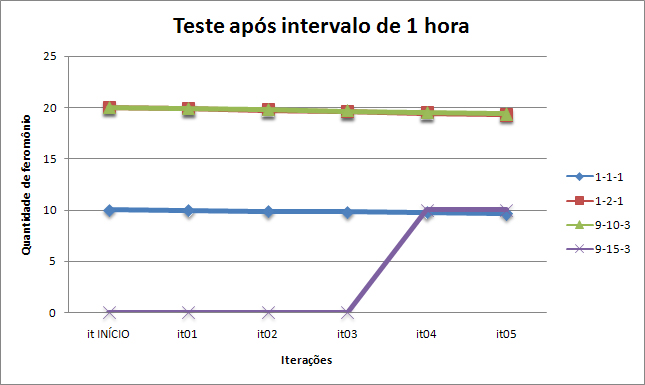
\includegraphics[width=10cm]{images/resultados/qtd_feromonio.jpg}
                \label{fig:qtd_feromonio}
                \caption{Gr�fico dos testes ap�s intervalo de 1 hora}
            \end{center}
        \end{figure}

\end{frame}

\begin{frame}[t,allowframebreaks]
\frametitle{Links acessados ap�s 10 horas do rein�cio dos registros}

        \begin{table}[H]
        \caption{Links acessados ap�s 10 horas do rein�cio dos registros}
        \label{tab:resultadotr10h}
        \tiny{
            \begin{center}
                \begin{tabular}{|c|c|r|r|r|r|r|r|}
                \hline
                \# & origem-destino-grupo & qf it1 & qf it2 & qf it3 & qf it4 & qf it5 \\
                \hline
                \textcolor[rgb]{0.31,0.51,0.74}{\textbf{1}} & \textcolor[rgb]{0.31,0.51,0.74}{\textbf{1-1-1}} & \textcolor[rgb]{0.31,0.51,0.74}{\textbf{9,31582}} & \textcolor[rgb]{0.31,0.51,0.74}{\textbf{8,67811}} & \textcolor[rgb]{0.31,0.51,0.74}{\textbf{8,08376}} & \textcolor[rgb]{0.31,0.51,0.74}{\textbf{7,5296}} & \textcolor[rgb]{0.31,0.51,0.74}{\textbf{7,01306}} \\
                \hline
                \textcolor[rgb]{0.75,0.31,0.30}{\textbf{2}} & \textcolor[rgb]{0.75,0.31,0.30}{\textbf{1-2-1}} &\textcolor[rgb]{0.75,0.31,0.30}{\textbf{18,63165}} & \textcolor[rgb]{0.75,0.31,0.30}{\textbf{17,35624}} & \textcolor[rgb]{0.75,0.31,0.30}{\textbf{16,16754}} & \textcolor[rgb]{0.75,0.31,0.30}{\textbf{15,05922}} & \textcolor[rgb]{0.75,0.31,0.30}{\textbf{14,02614}} \\
                \hline
                3 & 1-3-1 & 9,31691 & 8,68014 & 8,0866 & 7,53313 & 7,01717 \\
                \hline
                4 & 1-4-1 & 9,318 & 8,68217 & 8,08943 & 7,53664 & 7,02126 \\
                \hline
                5 & 1-5-2 & 9,32018 & 8,68624 & 8,09512 & 7,54371 & 7,02949 \\
                \hline
                6 & 5-6-2 & 18,64036 & 17,37247 & 16,19022 & 15,0874 & 14,05896 \\
                \hline
                7 & 5-7-2 & 9,32127 & 8,68827 & 8,09795 & 7,54723 & 7,03359 \\
                \hline
                8 & 5-8-2 & 9,32127 & 8,68827 & 8,09795 & 7,54723 & 7,03359 \\
                \hline
                9 & 1-9-3 & 20 & 19,99922 & 19,9977 & 19,99482 & 19,99089 \\
                \hline
                \textcolor[rgb]{0.61,0.73,0.35}{\textbf{10}} & \textcolor[rgb]{0.61,0.73,0.35}{\textbf{9-10-3}} & \textcolor[rgb]{0.61,0.73,0.35}{\textbf{18,64689}} & \textcolor[rgb]{0.61,0.73,0.35}{\textbf{17,38465}} & \textcolor[rgb]{0.61,0.73,0.35}{\textbf{16,20726}} & \textcolor[rgb]{0.61,0.73,0.35}{\textbf{15,10858}} & \textcolor[rgb]{0.61,0.73,0.35}{\textbf{14,08363}} \\
                \hline
                11 & 9-11-3 & 9,32454 & 8,69436 & 8,10647 & 7,55782 & 7,04593 \\
                \hline
                12 & 9-12-3 & 9,32454 & 8,69436 & 8,10647 & 7,55782 & 7,04593 \\
                \hline
                13 & 9-13-3 & 0 & 10 & 9,99963 & 9,99858 & 9,997 \\
                \hline
                14 & 9-14-3 & 0 & 0 & 10 & 9,99932 & 9,99811 \\
                \hline
                 \textcolor[rgb]{0.49,0.38,0.63}{\textbf{15}} &  \textcolor[rgb]{0.49,0.38,0.63}{\textbf{9-15-3}} &  \textcolor[rgb]{0.49,0.38,0.63}{\textbf{0}} &  \textcolor[rgb]{0.49,0.38,0.63}{\textbf{0}} &  \textcolor[rgb]{0.49,0.38,0.63}{\textbf{0}} &  \textcolor[rgb]{0.49,0.38,0.63}{\textbf{10}} &  \textcolor[rgb]{0.49,0.38,0.63}{\textbf{9,99947}} \\
                \hline
                16 & 9-16-3 & 0 & 0 & 0 & 0 & 10 \\
                \hline
                \end{tabular}
            \end{center}
        }
        \end{table}

        \begin{figure}[htb]
            \begin{center}
                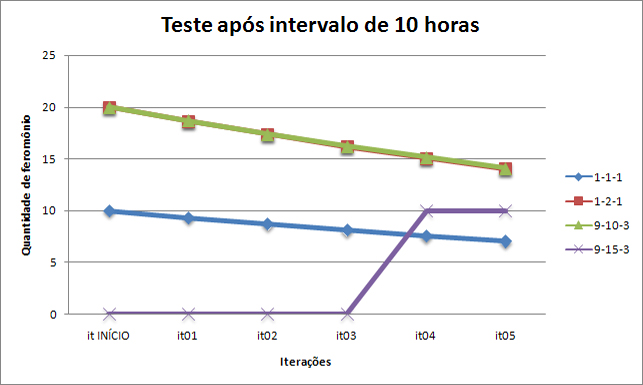
\includegraphics[width=10cm]{images/resultados/graf_teste10h.jpg}
                \label{fig:qtd_feromonio10h}
                \caption{Gr�fico dos testes ap�s intervalo de 10 horas}
            \end{center}
        \end{figure}
\end{frame}

\begin{frame}[t,allowframebreaks]
\frametitle{Links acessados ap�s 24 horas do rein�cio dos registros}

        \begin{table}[H]
        \caption{Links acessados ap�s 24 horas do rein�cio dos registros}
        \label{tab:resultadotr24h}
        \tiny{
            \begin{center}
                \begin{tabular}{|c|c|r|r|r|r|r|r|}
                \hline
                \# & origem-destino-grupo & qf it1 & qf it2 & qf it3 & qf it4 & qf it5 \\
                \hline
                \textcolor[rgb]{0.31,0.51,0.74}{\textbf{1}} & \textcolor[rgb]{0.31,0.51,0.74}{\textbf{1-1-1}} & \textcolor[rgb]{0.31,0.51,0.74}{\textbf{8,39057}} & \textcolor[rgb]{0.31,0.51,0.74}{\textbf{7,03988}} & \textcolor[rgb]{0.31,0.51,0.74}{\textbf{5,90639}} & \textcolor[rgb]{0.31,0.51,0.74}{\textbf{4,95517}} & \textcolor[rgb]{0.31,0.51,0.74}{\textbf{4,15693}} \\
                \hline
                \textcolor[rgb]{0.75,0.31,0.30}{\textbf{2}} & \textcolor[rgb]{0.75,0.31,0.30}{\textbf{1-2-1}} & \textcolor[rgb]{0.75,0.31,0.30}{\textbf{16,78114}} & \textcolor[rgb]{0.75,0.31,0.30}{\textbf{14,07976}} & \textcolor[rgb]{0.75,0.31,0.30}{\textbf{11,81278}} & \textcolor[rgb]{0.75,0.31,0.30}{\textbf{9,91034}} & \textcolor[rgb]{0.75,0.31,0.30}{\textbf{8,31387}} \\
                \hline
                3 & 1-3-1 & 8,39155 & 7,04153 & 5,90846 & 4,95749 & 4,15937 \\
                \hline
                4 & 1-4-1 & 8,39253 & 7,04317 & 5,91053 & 4,9598 & 4,16179 \\
                \hline
                5 & 1-5-2 & 8,3945 & 7,04647 & 5,91468 & 4,96445 & 4,16667 \\
                \hline
                6 & 5-6-2 & 16,78899 & 14,09293 & 11,82936 & 9,92889 & 8,33332 \\
                \hline
                4 & 5-7-2 & 8,39548 & 7,04812 & 5,91676 & 4,96677 & 4,1691 \\
                \hline
                7 & 5-8-2 & 8,39548 & 7,04812 & 5,91676 & 4,96677 & 4,1691 \\
                \hline
                8 & 1-9-3 & 20 & 19,99918 & 19,99758 & 19,99505 & 19,99151 \\
                \hline
                \textcolor[rgb]{0.61,0.73,0.35}{\textbf{10}} & \textcolor[rgb]{0.61,0.73,0.35}{\textbf{9-10-3}} & \textcolor[rgb]{0.61,0.73,0.35}{\textbf{16,79488}} & \textcolor[rgb]{0.61,0.73,0.35}{\textbf{14,10282}} & \textcolor[rgb]{0.61,0.73,0.35}{\textbf{11,84181}} & \textcolor[rgb]{0.61,0.73,0.35}{\textbf{9,94283}} & \textcolor[rgb]{0.61,0.73,0.35}{\textbf{8,34795}} \\
                \hline
                11 & 9-11-3 & 8,39842 & 7,05306 & 5,92298 & 4,97374 & 4,17642 \\
                \hline
                12 & 9-12-3 & 8,39842 & 7,05306 & 5,92298 & 4,97374 & 4,17642 \\
                \hline
                13 & 9-13-3 & 0 & 10 & 9,99961 & 9,99875 & 9,99739 \\
                \hline
                14 & 9-14-3 & 0 & 0 & 10 & 9,99953 & 9,99856 \\
                \hline
                 \textcolor[rgb]{0.49,0.38,0.63}{\textbf{15}} &  \textcolor[rgb]{0.49,0.38,0.63}{\textbf{9-15-3}} &  \textcolor[rgb]{0.49,0.38,0.63}{\textbf{0}} &  \textcolor[rgb]{0.49,0.38,0.63}{\textbf{0}} &  \textcolor[rgb]{0.49,0.38,0.63}{\textbf{0}} &  \textcolor[rgb]{0.49,0.38,0.63}{\textbf{10}} &  \textcolor[rgb]{0.49,0.38,0.63}{\textbf{9,99949}} \\
                \hline
                16 & 9-16-3 & 0 & 0 & 0 & 0 & 10 \\
                \hline
                \end{tabular}
            \end{center}
        }
        \end{table}

        \begin{figure}[htb]
            \begin{center}
                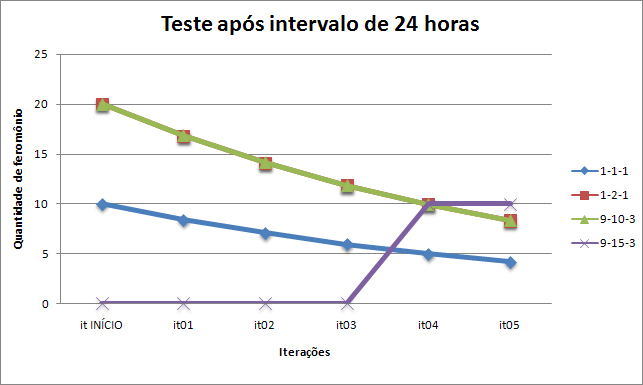
\includegraphics[width=10cm]{images/resultados/graf_teste24h.jpg}
                \label{fig:qtd_feromonio24h}
                \caption{Gr�fico dos testes ap�s intervalo de 24 horas}
            \end{center}
        \end{figure}
\end{frame}

\begin{frame}[t,allowframebreaks]
\frametitle{Diferen�a de ferom�nio nos testes efetuados}

        \begin{table}[H]
        \caption{Diferen�a de ferom�nio nos testes efetuados}
        \label{tab:testesdiferencas}
        \tiny{
            \begin{center}
            \begin{tabular}{|l|l|l|l|l|l|}
            \hline
            \multicolumn{1}{|c|}{Origem} & \multicolumn{1}{c|}{Destino} & \multicolumn{1}{c|}{Grupo} & \multicolumn{1}{c|}{dif 1h} & \multicolumn{1}{c|}{dif 10h} & \multicolumn{1}{c|}{dif 24h} \\
            \hline
            \multicolumn{1}{|c|}{1} & \multicolumn{1}{c|}{1} & \multicolumn{1}{c|}{1} & \multicolumn{1}{c|}{0,32939} & \multicolumn{1}{c|}{2,27586} & \multicolumn{1}{c|}{4,18039} \\
            \hline
            \multicolumn{1}{|c|}{1} & \multicolumn{1}{c|}{2} & \multicolumn{1}{c|}{1} & \multicolumn{1}{c|}{0,65876} & \multicolumn{1}{c|}{4,55171} & \multicolumn{1}{c|}{8,36076} \\
            \hline
            \multicolumn{1}{|c|}{1} & \multicolumn{1}{c|}{3} & \multicolumn{1}{c|}{1} & \multicolumn{1}{c|}{0,32939} & \multicolumn{1}{c|}{2,27586} & \multicolumn{1}{c|}{4,18039} \\
            \hline
            \multicolumn{1}{|c|}{1} & \multicolumn{1}{c|}{4} & \multicolumn{1}{c|}{1} & \multicolumn{1}{c|}{0,32939} & \multicolumn{1}{c|}{2,27586} & \multicolumn{1}{c|}{4,18039} \\
            \hline
            \multicolumn{1}{|c|}{1} & \multicolumn{1}{c|}{5} & \multicolumn{1}{c|}{2} & \multicolumn{1}{c|}{0,32939} & \multicolumn{1}{c|}{2,27586} & \multicolumn{1}{c|}{4,18039} \\
            \hline
            \multicolumn{1}{|c|}{5} & \multicolumn{1}{c|}{6} & \multicolumn{1}{c|}{2} & \multicolumn{1}{c|}{0,65876} & \multicolumn{1}{c|}{4,55171} & \multicolumn{1}{c|}{8,36076} \\
            \hline
            \multicolumn{1}{|c|}{5} & \multicolumn{1}{c|}{7} & \multicolumn{1}{c|}{2} & \multicolumn{1}{c|}{0,32939} & \multicolumn{1}{c|}{2,27586} & \multicolumn{1}{c|}{4,18039} \\
            \hline
            \multicolumn{1}{|c|}{5} & \multicolumn{1}{c|}{8} & \multicolumn{1}{c|}{2} & \multicolumn{1}{c|}{0,32939} & \multicolumn{1}{c|}{2,27586} & \multicolumn{1}{c|}{4,18039} \\
            \hline
            \multicolumn{1}{|c|}{1} & \multicolumn{1}{c|}{9} & \multicolumn{1}{c|}{3} & \multicolumn{1}{c|}{0,02329} & \multicolumn{1}{c|}{0,01679} & \multicolumn{1}{c|}{0,01317} \\
            \hline
            \multicolumn{1}{|c|}{9} & \multicolumn{1}{c|}{10} & \multicolumn{1}{c|}{3} & \multicolumn{1}{c|}{0,65876} & \multicolumn{1}{c|}{4,55171} & \multicolumn{1}{c|}{8,36076} \\
            \hline
            \multicolumn{1}{|c|}{9} & \multicolumn{1}{c|}{11} & \multicolumn{1}{c|}{3} & \multicolumn{1}{c|}{0,32939} & \multicolumn{1}{c|}{2,27586} & \multicolumn{1}{c|}{4,18039} \\
            \hline
            \multicolumn{1}{|c|}{9} & \multicolumn{1}{c|}{12} & \multicolumn{1}{c|}{3} & \multicolumn{1}{c|}{0,32939} & \multicolumn{1}{c|}{2,27586} & \multicolumn{1}{c|}{4,18039} \\
            \hline
            \end{tabular}
            \end{center}
        }
        \end{table}

        \begin{figure}[htb]
            \begin{center}
                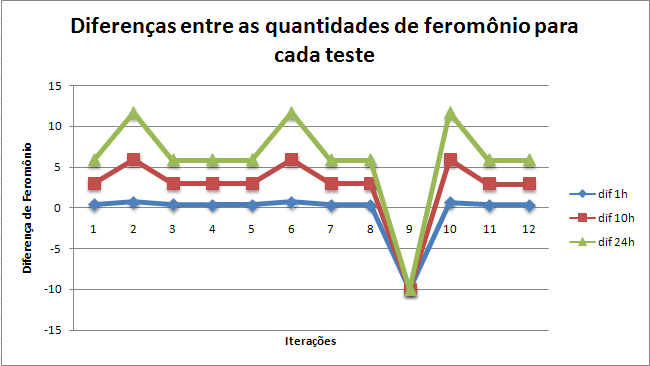
\includegraphics[width=10cm]{images/resultados/graf_diferencas.jpg}
                \label{fig:grafico:dif}
                \caption{Gr�fico indicativo com diferen�a de ferom�nio}
            \end{center}
        \end{figure}

\end{frame}
        % [ok]
        %%%%%%%%%%%%%%%%%%%%%%%%%%%%%%%%%%%%%%%%%%%%%%%%%
    % R E C U R S O S   C O M P U T A C I O N A I S %
    %%%%%%%%%%%%%%%%%%%%%%%%%%%%%%%%%%%%%%%%%%%%%%%%%

    \UTFPRchapter[cap:recursos]{RECURSOS COMPUTACIONAIS}

    Os recursos computacionais necess�rios s�o divididos entre:
    recursos dispon�veis para desenvolvimento e recursos
    necess�rios para utiliza��o descritos nas Se��es
    \ref{sec:recursosdeselvolvimento} e \ref{sec:recursosutilizacao}
    respectivamente.

    \UTFPRsection[sec:recursosdeselvolvimento]{RECURSOS DISPON�VEIS PARA DESENVOLVIMENTO}

    \UTFPRsubsection{Recursos de Hardware}

        \begin{enumerate}

        \item Microcomputador Desktop:

        \begin{enumerate}
            \item[a)] \emph{Processador:} AMD Athlon(tm) XP 2700+ (2.16 GHz);
            \item[b)] \emph{Mem�ria:} 512 MB;
            \item[c)] \emph{Armazenamento:} 120GB + 40GB.
        \end{enumerate}

        \item Microcomputador Notebook:

        \begin{enumerate}
            \item[a)] \emph{Modelo:} HP Pavilion dv1040;
            \item[b)] \emph{Processador:} Pentium M Centrino  (1.7 GHz);
            \item[c)] \emph{Mem�ria:} 512 MB;
            \item[d)] \emph{Armazenamento:} 60GB.
        \end{enumerate}

        \end{enumerate}

    \UTFPRsubsection{Recursos de \emph{Software}}

        \begin{enumerate}

        \item Sistemas Operacionais:

        \begin{enumerate}

            \item[a)] \emph{Windows XP Professional Edition SP2 PT-BR}:
            Sistema operacional utilizado com o
            microcomputador \emph{desktop};

            \item[b)] \emph{Windows XP Home Edition SP2 EN-US}:
            Sistema operacional utilizado com o
            microcomputador \emph{notebook}.

        \end{enumerate}

        \item Outros \emph{Softwares}:

        \begin{enumerate}
            \item[a)] \emph{Adobe Photoshop CS2}:
            Necess�rio para a constru��o dos \emph{layouts} (\emph{design}) do
            sistema;

            \item[b)] \emph{Adobe Acrobat Reader Professional 7.0}:
            Necess�rio para visualiza��o e altera��o
            do \UTFPRsigla{PDF}{\emph{Portable Document Format}} referente
            � monografia;

            \item[c)] \emph{Apache HTTP Server 1.3.33}:
            Servidor HTTP com suporte a linguagem PHP;

            \item[d)] \emph{Macromedia Dreamweaver 8.0}:
            Utilizado para a codifica��o e design do sistema;

            \item[e)] \emph{Visual Paradigm vers�o 5.2}:
            Utilizado para constru��o dos diagramas UML;

            \item[f)] \emph{Mozilla Firefox vers�o 1.5.0.5}:
            Navegador compat�vel com as especifica��es HTML 4.01,
            CSS 2, e possui suporte a JavaScript. Utilizado para
            testes no sistema;

            \item[g)] \emph{Internet Explorer 7.0}:
            Navegador compat�vel com as especifica��es HTML 4.01,
            CSS 2, e possui suporte a JavaScript. Utilizado para
            testes no sistema;

            \item[h)] \emph{winEdit 5.4}: Programa
            utilizado para codifica��o da monografia em \LaTeX;

            \item[i)] \emph{PostGreSQL 8.0.1}: Banco de
            dados utilizados neste trabalho;

            \item[j)] \emph{pgAdmin 1.4.2}: Ferramenta
            para gerenciamento do banco de dados PostGreSQL;

            \item[k)] \emph{ERwin 4.0}: Ferramenta para
            cria��o dos diagramas de entidades e relacionamentos;

            \item[l)] \emph{MiKTeX 2.5}: Compilador
            \LaTeX{} para Windows;

            \item[m)] \emph{PHP 5.1.4}: Linguagem de
            programa��o utilizada neste trabalho;


            \item[n)] \emph{LaTable 0.7.2}: Ferramenta
            para cria��o de tabelas;

            \item[o)] \emph{yEd Graph Editor 2.4.2.2}: Ferramenta
            para cria��o dos grafos.

        \end{enumerate}

        \end{enumerate}

    \UTFPRsection[sec:recursosutilizacao]{RECURSOS NECESS�RIOS PARA UTILIZA��O}

    \UTFPRsubsection{Usu�rio}

        Para utilizar o sistema, o usu�rio dever� possuir um microcomputador
        conectado a Internet com um navegador compat�vel com as
        especifica��es HTML 4.01, CSS 2 com suporte a
        JavaScript.

    \UTFPRsubsection{\emph{Website} Hospedeiro}

        O sistema elaborado, poder� ser implantado em \emph{websites} comuns
        que contemplem determinadas restri��es, tais como:

        \begin{itemize}
            \item O \emph{website} deve estar rodando em um navegador
                compat�vel com as especifica��es HTML 4.01, CSS 2, e
                deve possuir suporte a JavaScript;

            \item O \emph{website} deve suportar a linguagem de programa��o
            PHP;

            \item O \emph{website} deve possuir suporte ao banco de dados
            PostGreSQL 8.1, com disponibilidade de um banco de dados para o sistema a ser
            implantado.

        \end{itemize}
          % [ok]
        %%%%%%%%%%%%%%%%%%%%%%%%%
    % C R O N O G R A M A S %
    %%%%%%%%%%%%%%%%%%%%%%%%%

    \UTFPRchapter[cap:cronogramas]{CRONOGRAMAS}

Neste cap�tulo est�o descritos os cronogramas de trabalho, que est�o
divididos em: Cronograma das atividades desenvolvidas e Cronograma
da metodologia de desenvolvimento.

As atividades descritas correspondem a quesitos relativos ao
trabalho de conclus�o de curso e as disciplinas descrevem os fluxos
de trabalho descritos na Se��o \ref{sec:metodologia}.

%%%%%%%%%%%%%%%%%%%%%
% EXPLICAR ATIVIDADES E DISCIPLINAS
%%%%%%%%%%%%%%%%%%%%%

    \UTFPRsection{Atividades}

    \begin{itemize}
        \item[A1.] Reuni�o com orientador;
        \item[A2.] Pesquisa bibliogr�fica;
        \item[A3.] Reda��o da monografia;
        \item[A4.] Reda��o do artigo;
        \item[A5.] Defesa do trabalho de diploma��o;
    \end{itemize}

    \UTFPRsection{Disciplinas}

    \begin{itemize}
        \item[D1.] Requisitos;
        \item[D2.] An�lise;
        \item[D3.] Projeto;
        \item[D4.] Implanta��o;
        \item[D5.] Testes.
    \end{itemize}

    \UTFPRsection{Itera��es}

    \begin{itemize}
        \item[I1.] Itera��o \#1 $\rightarrow$ M�dulo: Computa��o de
        Ferom�nio; (Marcado com:
        {\textcolor[rgb]{0.00,0.00,0.46}{\textbullet}})
        \item[I2.] Itera��o \#2 $\rightarrow$ M�dulo: Adapta��o; (Marcado com:
        {\textcolor[rgb]{0.53,0.00,0.00}{\textbullet}})
        \item[I3.] Itera��o \#3 $\rightarrow$ M�dulo: Administra��o;
        (Marcado com:
        {\textcolor[rgb]{0.00,0.25,0.00}{\textbullet}})
    \end{itemize}


    As tarefas est�o divididas dentro do prazo previsto para a execu��o
    deste trabalho conforme as tabelas \ref{tab:cronograma1} e
    \ref{tab:cronograma2}.

    \begin{landscape}
        \begin{table}[H]
        \centering
             \begin{minipage}{\linewidth}
             {\footnotesize
                    \caption{Cronograma das atividades desenvolvidas}
                    \label{tab:cronograma1}
                    %\begin{tabular}{|p{2.6cm}|l|l|l|l|l|l|l|l|l|l|l|l|l|l|l|l|l|l|l|l|l|l|l|l|l|l|l|l|l|l|l|l|l|l|l|l|}
                    \begin{tabular}{|p{2cm}|l|l|l|l|l|l|l|l|l|l|l|l|l|l|l|l|l|l|l|l|l|l|l|l|l|l|l|l|l|l|l|l|l|l|l|l|l|l|l|l|}
                    \hline
                    \multicolumn{1}{|c|}{Atividades} & \multicolumn{4}{c|}{Dez/06} & \multicolumn{4}{c|}{Jan/07} & \multicolumn{4}{c|}{Fev/07} & \multicolumn{4}{c|}{Mar/07} & \multicolumn{4}{c|}{Abr/07} & \multicolumn{4}{c|}{Maio/07} & \multicolumn{4}{c|}{Jun/07} & \multicolumn{4}{c|}{Jul/07} & \multicolumn{4}{c|}{Ago/07} & \multicolumn{4}{c|}{Set/07} \\
                    \hline
                    & 1 & 2 & 3 & 4 & 1 & 2 & 3 & 4 & 1 & 2 & 3 & 4 & 1 & 2 & 3 & 4 & 1 & 2 & 3 & 4 & 1 & 2 & 3 & 4 & 1 & 2 & 3 & 4 & 1 & 2 & 3 & 4 & 1 & 2 & 3 & 4 & 1 & 2 & 3 & 4 \\
                    \hline
                    A1 &  & \textbullet &  & \textbullet &  & \textbullet &  & \textbullet &  &  &  &  & \textbullet &  &  &  &  &  &  & \textbullet &  & \textbullet &  & \textbullet &  & \textbullet &  & \textbullet &  & \textbullet &  &  &  &  & \textbullet & \textbullet &  &  &  &  \\
                    \hline
                    A2 &  &  &  &  &  &  &  &  & \textbullet &  & \textbullet &  &  &  &  & \textbullet &  & \textbullet &  & \textbullet &  &  &  &  & \textbullet & \textbullet & \textbullet & \textbullet & \textbullet & \textbullet & \textbullet & \textbullet & \textbullet &  &  &  &  &  &  &  \\
                    \hline
                    A3 &  &  &  &  &  &  &  &  &  &  &  &  &  &  &  &  &  &  &  &  &  &  &  & \textbullet &  &  &  &  &  &  & \textbullet & \textbullet & \textbullet & \textbullet & \textbullet & \textbullet & \textbullet &  &  &  \\
                    \hline
                    A4 &  &  &  &  &  &  &  &  &  &  &  &  &  &  &  &  &  &  &  &  &  &  &  &  & \textbullet & \textbullet & \textbullet & \textbullet & \textbullet & \textbullet &  &  &  &  &  &  &  &  &  &  \\
                    \hline
                    A5 &  &  &  &  &  &  &  &  &  &  &  &  &  &  &  &  &  &  &  &  &  &  &  &  &  &  &  &  &  &  &  &  &  &  &  &  &  & \textbullet &  &  \\
                    \hline
                    \end{tabular}
             }
             \end{minipage}
        \end{table}

        \begin{table}[H]
        \centering
             \begin{minipage}{\linewidth}
             {\footnotesize
                    \caption{Cronograma da metodologia de desenvolvimento}
                    \label{tab:cronograma2}
                    %\begin{tabular}{|p{2.6cm}|l|l|l|l|l|l|l|l|l|l|l|l|l|l|l|l|l|l|l|l|l|l|l|l|l|l|l|l|l|l|l|l|l|l|l|l|}
                    \begin{tabular}{|p{2cm}|l|l|l|l|l|l|l|l|l|l|l|l|l|l|l|l|l|l|l|l|l|l|l|l|l|l|l|l|l|l|l|l|l|l|l|l|l|l|l|l|}
                    \hline
                    \multicolumn{1}{|c|}{Disciplinas} & \multicolumn{4}{c|}{Dez/06} & \multicolumn{4}{c|}{Jan/07} & \multicolumn{4}{c|}{Fev/07} & \multicolumn{4}{c|}{Mar/07} & \multicolumn{4}{c|}{Abr/07} & \multicolumn{4}{c|}{Maio/07} & \multicolumn{4}{c|}{Jun/07} & \multicolumn{4}{c|}{Jul/07} & \multicolumn{4}{c|}{Ago/07} & \multicolumn{4}{c|}{Set/07} \\
                    \hline
                    & 1 & 2 & 3 & 4 & 1 & 2 & 3 & 4 & 1 & 2 & 3 & 4 & 1 & 2 & 3 & 4 & 1 & 2 & 3 & 4 & 1 & 2 & 3 & 4 & 1 & 2 & 3 & 4 & 1 & 2 & 3 & 4 & 1 & 2 & 3 & 4 & 1 & 2 & 3 & 4 \\
                    \hline
                    D1 &  &  & {\textcolor[rgb]{0.00,0.00,0.46}{\textbullet}} & {\textcolor[rgb]{0.00,0.00,0.46}{\textbullet}} & {\textcolor[rgb]{0.00,0.00,0.46}{\textbullet}} & {\textcolor[rgb]{0.00,0.00,0.46}{\textbullet}} &  &  &  & {\textcolor[rgb]{0.53,0.00,0.00}{\textbullet}} & {\textcolor[rgb]{0.53,0.00,0.00}{\textbullet}} & {\textcolor[rgb]{0.53,0.00,0.00}{\textbullet}} &  &  &  &  &  &  &  & {\textcolor[rgb]{0.00,0.25,0.00}{\textbullet}} & {\textcolor[rgb]{0.00,0.25,0.00}{\textbullet}} &  &  &  &  &  &  &  &  &  &  &  &  &  &  &  &  &  &  &  \\
                    \hline
                    D2 &  &  &  &  & {\textcolor[rgb]{0.00,0.00,0.46}{\textbullet}} & {\textcolor[rgb]{0.00,0.00,0.46}{\textbullet}} &  &  &  &  &  & {\textcolor[rgb]{0.53,0.00,0.00}{\textbullet}} &  &  &  &  &  &  &  &  &  & {\textcolor[rgb]{0.00,0.25,0.00}{\textbullet}} &  &  &  &  &  &  &  & {\textcolor[rgb]{0.00,0.25,0.00}{\textbullet}} &  &  &  &  &  &  &  &  &  &  \\
                    \hline
                    D3 &  &  &  &  &  & {\textcolor[rgb]{0.00,0.00,0.46}{\textbullet}} &  &  &  &  &  &  & {\textcolor[rgb]{0.53,0.00,0.00}{\textbullet}} &  &  &  &  &  &  &  &  & {\textcolor[rgb]{0.00,0.25,0.00}{\textbullet}} &  &  &  &  &  &  &  & {\textcolor[rgb]{0.00,0.25,0.00}{\textbullet}} &  &  &  &  &  &  &  &  &  &  \\
                    \hline
                    D4 &  &  &  &  & {\textcolor[rgb]{0.00,0.00,0.46}{\textbullet}} & {\textcolor[rgb]{0.00,0.00,0.46}{\textbullet}} & {\textcolor[rgb]{0.00,0.00,0.46}{\textbullet}} & {\textcolor[rgb]{0.00,0.00,0.46}{\textbullet}} & {\textcolor[rgb]{0.00,0.00,0.46}{\textbullet}} & {\textcolor[rgb]{0.00,0.00,0.46}{\textbullet}} & {\textcolor[rgb]{0.00,0.00,0.46}{\textbullet}} &  & {\textcolor[rgb]{0.53,0.00,0.00}{\textbullet}} & {\textcolor[rgb]{0.53,0.00,0.00}{\textbullet}} & {\textcolor[rgb]{0.53,0.00,0.00}{\textbullet}} & {\textcolor[rgb]{0.53,0.00,0.00}{\textbullet}} & {\textcolor[rgb]{0.53,0.00,0.00}{\textbullet}} & {\textcolor[rgb]{0.53,0.00,0.00}{\textbullet}} & {\textcolor[rgb]{0.53,0.00,0.00}{\textbullet}} &  &  & {\textcolor[rgb]{0.00,0.25,0.00}{\textbullet}} &  &  &  &  &  &  &  & {\textcolor[rgb]{0.00,0.25,0.00}{\textbullet}} & {\textcolor[rgb]{0.00,0.25,0.00}{\textbullet}} & {\textcolor[rgb]{0.00,0.25,0.00}{\textbullet}} &  &  &  &  &  &  &  &  \\
                    \hline
                    D5 &  &  &  &  &  &  &  &  & {\textcolor[rgb]{0.00,0.00,0.46}{\textbullet}} &  & {\textcolor[rgb]{0.00,0.00,0.46}{\textbullet}} &  &  &  &  &  & {\textcolor[rgb]{0.53,0.00,0.00}{\textbullet}} &  & {\textcolor[rgb]{0.53,0.00,0.00}{\textbullet}} &  &  & {\textcolor[rgb]{0.00,0.25,0.00}{\textbullet}} &  &  &  &  &  &  &  &  & {\textcolor[rgb]{0.00,0.25,0.00}{\textbullet}} & {\textcolor[rgb]{0.00,0.25,0.00}{\textbullet}} &  &  &  &  &  &  &  &  \\
                    \hline
                    \end{tabular}
             }
             \end{minipage}
        \end{table}

    \end{landscape}
       % [ok]
    \section[Conclus�o]{Conclus�o}

\begin{frame}
    \frametitle{Conclus�o}
    \begin{itemize}
		\item proposta de um trabalho para execu��o de fluxos de trabalho cient�ficos;
		\item t�cnicas de planejamento:
		\begin{itemize}
			\item tempo de execu��o: estimado fornecido pelo usu�rio;
			\item coeficiente de tempo: execu��es anteriores;
			\item situa��o atual do ambiente distribu�do;
		\end{itemize}
		\item coeficiente de custos: utilizado pelo planejador para criar planos de execu��o;
		\item modulariza��o dos componentes do modelo;
		\item cen�rio flex�vel e expans�vel;
		\item modifica��o do \emph{PeerUnit}: gerenciador de execu��o;
		\item defini��o de um modelo de custos;
		\item uma limita��o do modelo: fluxos c�clicos;
		\begin{itemize}
			\item alternativa parcial: encapsular fluxo de trabalho (m�ltiplas entradas e sa�da de dados);
		\end{itemize}
	\end{itemize}
\end{frame}

\begin{frame}
    \frametitle{Trabalhos Futuros}
    \begin{itemize}
		\item refinamento do \emph{Or�culoDeMetaDados};
		\item utiliza��o de outras m�tricas:
		\begin{itemize}
			\item minimiza��o de gasto de energia;
			\item maximiza��o da utiliza��o de recursos;
		\end{itemize}
		\item m�todo de difus�o inteligente: capaz de analisar o plano e propagar os dados apenas para os n�s que utilizar�o tais dados;
		\item planejador capaz de escolher a melhor implementa��o de um operador para o plano a ser gerado:
		\item paraleliza��o por plano:
		\begin{itemize}
			\item n�o se fixa uma quantidade de n�s para cada fluxo de trabalho;
			\item de acordo com informa��es do \emph{Or�culoDeMetadados} planejador define o n�mero adequado para a paraleliza��o;
			\item necess�ria adapta��o do m�todo de tradu��o (considerar os n�s dispon�veis para cada tarefa);
		\end{itemize}
	\end{itemize}
\end{frame}

    %%%%%%%%%%%%%%%%%%%%%%%%%%%%%%%%%%%%%%%%%%%%%%
    % E L E M E N T O S  P � S - T E X T U A I S %
    %%%%%%%%%%%%%%%%%%%%%%%%%%%%%%%%%%%%%%%%%%%%%%

    \UTFPRbibliographystyle{abnt-alf}

    \UTFPRbibliografia{bib/bibliografia}

    \UTFPRapendice
    \chapter{GLOSS�RIO}\label{ape:glossario}

\par
Este documento apresenta um gloss�rio com os termos importantes
utilizados no projeto de desenvolvimento da ferramenta de apoio ao
desenvolvimento global de \emph{software}.

\UTFPRsection{INTRODU��O}

O presente documento prov� um conjunto de defini��es importantes
para evitar ambig�idades, de forma que os leitores compreendam as
terminologias espec�ficas utilizadas nesse projeto.

\UTFPRsection{OBJETIVO}

Auxiliar os leitores na compreens�o de alguns termos t�cnicos
descritos durante o documento.

\UTFPRsection{ESCOPO}

Este gloss�rio est� associado ao projeto de desenvolvimento de uma
ferramenta de apoio a navega��o, utilizando conceitos de hiperm�dia
adaptativa e otimiza��o por col�nia de formigas.

%\UTFPRsection{ORGANIZA��O DO DOCUMENTO}
%
%A Se��o \ref{sec:glodef} apresenta os termos relevantes ao
%desenvolvimento desta ferramenta e suas defini��es. A listagem
%encontra-se em ordem alfab�tica para facilitar o acesso a palavras
%espec�ficas.

\newpage

\UTFPRsection[sec:glodef]{DEFINI��ES}

%%%%%%%%%%%%%%%%%%%%%%%%%%%%%%%%%%%%%%%%%%%%%%%%%%%%%%%%%%%%%%%%%%

\UTFPRglossario{ajax}{Asynchronous Javascript And XML. � o uso
sistem�tico de tecnologias providas por navegadores, Javascript e
XML, para tornar p�ginas mais interativas com o usu�rio.}

\UTFPRglossario{algoritmo}{algoritmo � uma sequ�ncia finita e n�o
amb�gua de instru��es comput�veis para solucionar um problema.}

\UTFPRglossario{\emph{array}}{Matriz, tabela, conjunto de objetos
que est� organizado geometricamente, utilizado para descrever
estruturas repetitivas ou sistem�ticas dentro do sistema.}

\UTFPRglossario{\emph{frame}}{(Moldura ou quadro) S�o subdivis�es da
janela principal do navegador ou \emph{browser}. Cada subdivis�o
funciona como uma pequena janela, exibindo conte�dos independentes.
Os criadores de \emph{sites} da \emph{web} utilizam este recurso
quando � necess�rio exibir muitas informa��es de uma s� vez. Em
comunica��o de dados, � um grupo de \emph{bits} que forma um bloco
adequado � transmiss�o como unidade.}

\UTFPRglossario{\emph{framework}}{Cole��o abstra�da de classes,
interfaces e padr�es, dedicados a resolver uma fam�lia de problemas
semelhantes, atrav�s de uma arquitetura flex�vel e extens�vel.}

\UTFPRglossario{grafo}{Em matem�tica e ci�ncia da computa��o, grafo
� o objeto b�sico de estudo da teoria dos grafos. Tipicamente, um
grafo � representado como um conjunto de pontos (v�rtices) ligados
por retas (as arestas). Dependendo da aplica��o, as arestas podem
ser direcionadas, e s�o representadas por "setas".}

\UTFPRglossario{heur�stica}{M�todo de solu��o de problemas indutivo
baseado em regras derivadas do senso comum ou da experi�ncia de um
modelo te�rico da matem�tica. Fornece uma base geral para a solu��o
de problemas, contrastando com abordagens estritamente algor�tmicas,
que nunca variam.}

\UTFPRglossario{\emph{hiperlinks}}{S�o palavras ou ilustra��es
pr�-estabelecidas como pontos de saltos. Quando clicadas, provocam a
transfer�ncia para outro assunto ou p�gina \emph{web}.}

\UTFPRglossario{hiperm�dia}{Documento que cont�m imagens, sons,
textos e v�deos, utilizando liga��es de hipertextos para permitir o
acesso para outro documento.}

\UTFPRglossario{hipertextos}{Em computa��o, hipertexto � um sistema
para a visualiza��o de informa��o cujos documentos cont�m
refer�ncias internas para outros documentos (chamadas de
\emph{hiperlinks} ou, simplesmente, \emph{links}), e para a f�cil
publica��o, atualiza��o e pesquisa de informa��o.}

\UTFPRglossario{javascript}{Linguagem de programa��o, criada pela
Netscape, que funciona interativamente com o c�digo HTML, aumentando
os recursos do navegador.}

\UTFPRglossario[\emph{links}]{\emph{links}}{O mesmo que
\emph{hiperlinks}.}

\UTFPRglossario{multim�dia}{Tecnologia que permite combinar, em um
�nico programa ou m�todo de acesso (rede, CD-ROM, etc.), informa��es
em diferentes meios, tais como texto, imagens est�ticas e din�micas,
clipes de �udio e de v�deo. Inclui fun��es de interatividade, ou
seja, a possibilidade do usu�rio interagir com o programa na forma
de um di�logo bidirecional. Tamb�m chamado de multimeios.}

\UTFPRglossario{navega��o}{Ato de conectar-se a diferentes
computadores da rede distribu�dos pelo mundo, usando as facilidades
providas por ferramentas como browsers \emph{web}. O navegante da
rede realiza uma "viagem" virtual explorando o ciberespa�o, da mesma
forma que o astronauta explora o espa�o sideral.}

\UTFPRglossario{nodo}{Um Nodo ou n� representa cada ponto de
inter-conex�o com uma estrutura ou rede, independente da fun��o do
equipamento representado por ele.}

\UTFPRglossario{POSIX}{POSIX � o nome de uma familia de normas
relacionadas definidas pelo IEEE e designada formalmente por IEEE
1003. A designa��o internacional da norma � ISO/IEC 9945. A
normaliza��o das especifica��es POSIX surgiram de um projeto,
iniciado por volta de 1985, que tinha como objetivo normalizar a
interface de programa��o de aplica��es para \emph{software}
desenhado para correr em variantes do sistema operativo UNIX.}

\UTFPRglossario{processo unificado}{O Processo Unificado (UP) de
desenvolvimento de sistemas combina os ciclos interativo e
incremental para a constru��o de \emph{softwares}. � fundamental na
vis�o de que o avan�o de um projeto deve estar baseado na constru��o
de artefatos de \emph{software}, e n�o apenas em documenta��o.}

\UTFPRglossario{\emph{software}}{S�o os programas, dados e rotinas
desenvolvidos para computadores. Os programas de \emph{software}
precisam ser instalados nos computadores para que eles passem a
desempenhar determinadas fun��es.}

\UTFPRglossario{web}{Termo usado para representar a grande rede de
informa��es de multim�dia da Internet}

\UTFPRglossario{\emph{website}}{Um s�tio, mais conhecido pelo
equivalente ingl�s \emph{site}, de \emph{website} ou \emph{web
site}, � uma cole��o de p�ginas \emph{web}, isto �, de documentos
acess�veis atrav�s da \emph{World Wide Web}, na Internet.}

\UTFPRglossario{\emph{workflows}}{Fluxo de trabalho, ou seja, um
sistema de informa��o que gere um conjunto de tarefas tipicamente
rotineiras, assegurando o controlo das entregas, dos tempos de
resposta, o \emph{time-stamping} (a que horas determinada tarefa foi
executada) a n�o repudia��o, a pesquisa de informa��o eo arquivo.}

\UTFPRimprimeGlossario
         % [ok]
    \chapter{PERGUNTAS FREQ�ENTES}\label{ape:faq}

Para ajudar o usu�rio a compreender melhor a utiliza��o do sistema
se criou uma seq��ncia de \UTFPRsigla{FAQ}{\emph{Frequently Asked
Question}}:

\paragraph{O que � OriAnt?}

    \hspace{1cm}

    OriAnt � um sistema computacional baseado no comportamentos das
    col�nias de formigas reais. O OriAnt funciona como um
    hospedeiro em uma p�gina \emph{web} e basicamente coleta as
    informa��es dos \emph{links} acionados pelos usu�rios para orientar os
    usu�rios na navega��o.

\paragraph{Por que o nome OriAnt?}

    \hspace{1cm}

    A palavra "Ant"{} em ingl�s significa formiga, a jun��o com o
    prefixo "Ori"{} forma a palavra Oriente, que significa orienta��o,
    dire��o.

\paragraph{Por que escolher um grupo?}

    \hspace{1cm}

    O grupo selecionado pelo usu�rio � de suma import�ncia, pois,
    � baseado no hist�rico de usu�rios que acessaram o mesmo grupo
    que o sistema consegue gerar os \emph{links} mais relevantes.

\paragraph{Caso eu n�o escolha um grupo o sistema funcionar�?}

    \hspace{1cm}

    N�o, o sistema s� entrar� em a��o quando um grupo for
    selecionado.

\paragraph{Eu posso escolher outro grupo durante a navega��o?}

    \hspace{1cm}

    Sim, voc� pode trocar de grupo a qualquer momento, basta clicar
    no �cone alterar grupo, que fica ao lado do grupo escolhido.

\paragraph{Ao clicar nos links da camada OriAnt, ainda continuarei no
    site em que estou navegando?}

    \hspace{1cm}

    Sim, os \emph{links} da camada OriAnt s� apontam para a p�gina atual
    que voc� est� navegando, apenas os \emph{links} de idioma e ajuda
    apontam para uma sub-p�gina do OriAnt.

\paragraph{Outros usu�rios podem ver as p�ginas que eu acesso?}

    \hspace{1cm}

    N�o, o sistema n�o cadastra os usu�rios, a identidade do usu�rio
    � mantida em sigilo.

\paragraph{Os tipos de orienta��o interferem no \emph{link} clicado?}

    \hspace{1cm}

    N�o, os tipos de orienta��o apenas exibem as sugest�es de forma
    diferente, n�o interferem na computa��o dos cliques.

\paragraph{Intera��es com a p�gina como: Coment�rios, Avalia��es e
    Contatos interferem na computa��o dos cliques?}

    \hspace{1cm}

    Esse clique ser� computado, somente se a intera��o o redirecionar para outra
    p�gina.

\paragraph{Onde o OriAnt armazena as informa��es?}

    \hspace{1cm}

    O OriAnt requer um banco de dados PostGreSQL 8.1 ou superior
    parar armazenar os dados.

\paragraph{O OriAnt funciona para um \emph{site} externo ao dom�nio, por
    exemplo, eu poderia usar o OriAnt no site da UOL?}

    \hspace{1cm}

    N�o, por motivos de seguran�a e limita��es, o sistema OriAnt s� funciona em um
    \emph{site} de mesmo dom�nio.

\paragraph{O website hospedeiro poder� utilizar banco de dados?}

    \hspace{1cm}

    Sim, poder� utiliza-lo.

\paragraph{O \emph{website} hospedeiro deve utilizar o banco de dados
PostGreSQL?}

    \hspace{1cm}

    N�o, o banco de dados n�o precisa ser o mesmo, entretanto,
    deve-se ter suporte a esse banco de dados.

\paragraph{O \emph{website} hospedeiro pode conter \emph{frames}?}

    \hspace{1cm}

    N�o, o sistema OriAnt � um \emph{frame} e n�o suporta sub
    \emph{frames}.

\paragraph{O website poder� utilizar javascript para redirecionar
um \emph{link}?}

    \hspace{1cm}

    N�o, a p�gina deve utilizar apenas \emph{links} para navega��o. Links que tiverem fun��es javascripts ser�o desconsiderados.

\paragraph{Deve-se ter os \emph{cookies} habilitado para navegar no
sistema?}

    \hspace{1cm}

    Sim, as informa��es escolhidas pelo usu�rio s�o armazenadas em \emph{cookies} e em sess�es.

\paragraph{Qual a diferen�a entre os tipos de orienta��o?}

    \hspace{1cm}

    Os tipos de orienta��o mostram v�rias formas de se atingir a
    p�gina mais relevante. S�o elas:

            \subparagraph{\emph{Disposi��o objetiva}:}

            \hspace{1cm}

            Mostra qual � a p�gina
            alvo. Essa � a p�gina que em m�dia foi mais visitada pelos
            outros elementos de um mesmo grupo.

            \subparagraph{\emph{Disposi��o orientada}:}

            \hspace{1cm}

            Mostra qual o caminho que se
            deve seguir para chegar at� a p�gina alvo. Esse caminho �
            tra�ado com base no hist�rico dos caminhos percorridos de usu�rios do mesmo grupo.

            \subparagraph{\emph{Disposi��o relacionada}:}

            \hspace{1cm}

            Mostra quais os links mais visitados pelos usu�rios de seu
            grupo. Al�m da p�gina alvo outras p�ginas tamb�m podem
            interessar o usu�rio de determinado grupo, assim ao
            selecionar a exibi��o por assuntos relacionados, obt�m-se
            uma lista das p�ginas mais relevantes para determinado
            grupo.

\paragraph{Qual a diferen�a entre os contextos de orienta��o?}

            \subparagraph{\emph{Essa P�gina}:}

            \hspace{1cm}

            Quando essa op��o est�
            selecionada, a disposi��o toma como contexto a p�gina
            atual, ou seja, a partir da p�gina atual qual ser� a
            pr�xima p�gina mais relevante.

            \subparagraph{\emph{Todas as P�ginas}:}

            \hspace{1cm}

            Quando essa op��o est�
            selecionada a disposi��o toma como contexto todas as p�ginas do sistema,
            ou seja, dentre todas as p�ginas qual � a p�gina mais
            relevante.
               % [ok]
    \chapter{APRESENTA��O DA CAMADA ORIANT}\label{ape:apreoriant}

\UTFPRfigura{width=16cm}{oriant/grupos.jpg}{Disposi��o dos grupos de
interesse}{fig:grupo}

\UTFPRfigura{width=16cm}{oriant/objetiva.jpg}{Disposi��o
objetiva}{fig:objetiva}

\UTFPRfigura{width=16cm}{oriant/orientada.jpg}{Disposi��o
orientada}{fig:orientada}

\UTFPRfigura{width=16cm}{oriant/relacionada.jpg}{Disposi��o
relacionada}{fig:relacionada}

\UTFPRfigura{width=16cm}{oriant/roxo.jpg}{Pele roxa}{fig:skinroxo}

\UTFPRfigura{width=16cm}{oriant/amarelo.jpg}{Pele
amarela}{fig:skinamarelo}

\UTFPRfigura{width=16cm}{oriant/idioma.jpg}{Sistema em
ingl�s}{fig:idioma}
      % [ok]
    %%%%%%%%%%%%%%%%%%%%%%%%%%%%%%%%%%%%%%%%%%%%%%%
% S U B S I S T E M A   P A R A   T E S T E S %
%%%%%%%%%%%%%%%%%%%%%%%%%%%%%%%%%%%%%%%%%%%%%%%

\UTFPRchapter[cap:subsistema]{SUBSISTEMA PARA TESTES}

O sistema proposto n�o poderia funcionar sem um \emph{website}
hospedeiro. Por tanto, foi desenvolvido um subsistema para testes
denominado \emph{Go!} Not�cias, que tamb�m implementa o
\emph{framework} descrito no Cap�tulo \ref{cap:framework} e utiliza
seus recursos para exibi��o de not�cias no formato RSS. A Figura
\ref{fig:subPgPrincipal} apresentada no Ap�ndice
\ref{ape:apresubsistema} mostra a p�gina principal do subsistema.

O subsistema possui a funcionalidade b�sica de administra��o, em que
� poss�vel gerenciar graficamente um menu em formato de grafo. Os
nodos que n�o possuem filhos (nodo folha) redirecionam o usu�rio
para uma lista de not�cias extra�das do RSS cadastrado nesse nodo do
grafo e os nodos que possuem filhos abrem sua ramifica��o com os
nodos dispon�veis.

A Figura \ref{fig:subMenuAdmin} do ap�ndice \ref{ape:apresubsistema}
ilustra a disposi��o do menu.

\begin{figure}[!htb]
\Tree [.$NP$ $NF$ [.$NPF$ $NF$ ] $NF$ ] \caption{Exemplo de grafo
gerado pelo subsistema} \label{fig:figuraArvoreSubSistema}
\end{figure}

Na Figura \ref{fig:figuraArvoreSubSistema}, $NP$ representa um Nodo
Pai, $NF$ um nodo filho e $NPF$ um nodo filho e tamb�m pai.

Na lista de not�cias exibida, ao se escolher um $NF$ � poss�vel
observar alguns dados iniciais da not�cia como: t�tulo, nota (m�dia
entre as avalia��es efetuadas), n�mero de coment�rios, \emph{link}
direto para a fonte da not�cia e um \emph{link} para ver os detalhes
dessa not�cia. Ao se optar por visualizar os detalhes da not�cia �
poss�vel ler um resumo da not�cia em quest�o, visualizar os
\emph{links} relacionados, avaliar ou comentar a not�cia.

O sistema foi programado para extrair os \emph{feeds}
automaticamente da fonte RSS a cada intervalo de tempo, tornando o
sistema constantemente atualizado com as �ltimas not�cias.

    \UTFPRsection[sec:submer]{Modelo Relacional}

    Para melhor ilustrar o subsistema \emph{Go}! Not�cias, pode-se
    observar seu modelo relacional, na Figura \ref{fig:mergo}

    \UTFPRfigura{width=8cm}{diagramas/mergo.jpg}{Modelo Relacional do Sub-sistema \emph{Go}! Not�cias}{fig:mergo}

    As tabelas "Avaliacao" e "Comentarios"{} n�o se relacionam diretamente com
    a not�cia em quest�o, esse relacionamento � feito pela URL (campo "pg") da
    not�cia. Esta forma de funcionamento, foi criado para
    que esses dois sistemas possam ser implantados em qualquer
    \emph{website} que utilize um sistema de not�cias.

    A tabela "NoticiasRSS"{} representa o menu em formato de grafo, um
    auto-relacionamento � criado para identificar qual nodo � seu pai,
    dessa forma, todos os nodos est�o em uma �nica tabela que � montada
    de forma recursiva. O campo ordem armazena uma \emph{string} que
    representar� a ordem desse nodo no grafo.

    A tabela Admin armazena as informa��es para administra��o do
    sistema.

    \UTFPRsection{Sistema de Avalia��o}

    O sistema de avalia��o foi criado para que os usu�rios possam
    avaliar o conte�do de uma p�gina qualquer. Com os recursos AJAX, a
    avalia��o se torna agrad�vel pois n�o � necess�rio que o usu�rio
    aguarde o recarregamento da p�gina. A metodologia de avalia��o �
    definida por uma escala de pontua��o que vai de 1 a 10, como se pode
    observar na Figura \ref{fig:aval}.

    \UTFPRfigura{width=5cm}{sub/aval.jpg}{Sistema de
    avalia��o}{fig:aval}

    A colabora��o entre os usu�rios na avalia��o, tamb�m � uma forma
    interessante e mais simples de se implantar a classifica��o
    adaptativa, t�cnica de navega��o adaptativa, explanada no Cap�tulo~\ref{cap:fundamentos}.

    \UTFPRsection{Sistema de Coment�rios}

    O sistema de coment�rios permite que os usu�rios troquem opini�es
    sobre o conte�do de determinada not�cia. O sistema tamb�m foi
    desenvolvido com o AJAX e possibilita o envio do coment�rio sem a
    necessidade de atualiza��o da p�gina. Um exemplo dos coment�rios
    pode ser observado na Figura \ref{fig:come}.

    \UTFPRfigura{width=8cm}{sub/come.jpg}{Sistema de
    coment�rios}{fig:come}

    Este recurso foi implementada a t�cnica de nota��o adaptativa
    explanada no Cap�tulo \ref{cap:fundamentos}.


    A Figura \ref{fig:subDetalhesNot} do ap�ndice \ref{ape:apresubsistema}
    mostra os sistemas de avalia��o e coment�rio implantados no
    subsistema.
        % [ok]
    \chapter{IMPLEMENTA��O DOS RECURSOS DE DESENVOLVIMENTO}\label{ape:codtableless}

Para demonstrar a versatilidade da utiliza��o dos recursos citados
no Cap�tulo \ref{cap:desenvolvimento}, est�o transcritos c�digos
efetivamente utilizados no projeto.

\UTFPRsection[ape:tableless]{TABLELESS}

O C�digo \ref{cod:oriantHTML} transcreve as linhas do arquivo
\texttt{oriant.html} que abriga a camada principal do sistema.

\texttt{\lstinputlisting[language=HTML, label=cod:oriantHTML,
caption={C�digo do arquivo oriant.html}]{cods/oriAntHTML.txt}}

No C�digo \ref{cod:oriantHTML} as linhas que est�o entre as tags
"$<! --$"{} e "$-- >$"{} s�o coment�rios utilizados na substitui��o
de tags no sistema de \emph{templates} implementado, e as vari�veis
s�o definidas por uma palavra entre colchetes \{\}, (ver Se��o
\ref{subsec:pear}). A linha 9 faz liga��o do c�digo HTML � um c�digo
CSS, nota-se que na URL h� uma vari�vel (\texttt{\emph{skin}}) que
ser� substitu�da pelo nome do \emph{template} de interface
selecionado. O trecho de c�digo localizado entre as linhas 33 e 69
monta o \emph{layout} da camada OriAnt, � poss�vel observar que n�o
h� a utiliza��o da \emph{tag} "\emph{table}"{} para a composi��o do
\emph{layout}.

O C�digo \ref{cod:oriAntCSS} transcreve as linhas do arquivo
\texttt{oriAnt.css} que � uma das folhas de estilo invocada pelo
C�digo \ref{cod:oriantHTML}.

\texttt{\lstinputlisting[language=HTML, label=cod:oriAntCSS,
caption={C�digo do arquivo oriAnt.css}]{cods/oriAntCSS.txt}}

O C�digo \ref{cod:oriAntCSS} formata as \emph{tags} do arquivo
\texttt{oriant.html} compondo o \emph{layout} da camada. Para
alterar as cores e figuras do \emph{layout} basta a substitui��o
desse arquivo.

\UTFPRsection[ape:rss]{RSS}

O C�digo \ref{cod:rss} exemplifica a especifica��o RSS mencionada na
Se��o \ref{subsec:rss}.

\texttt{\lstinputlisting[language=HTML, label=cod:rss,
caption={Exemplo de RSS utilizado no subsistema para
testes}]{cods/rss.txt}}

\UTFPRsection[ape:ajax]{AJAX}

Para solidificar a utiliza��o da tecnologia AJAX no sistema
proposto, transcreve-se parte dos c�digos para a obten��o dos grupos
de interesses do sistema.

O trecho de C�digo \ref{cod:ajaxPHP} mostra al�m das configura��es
do \emph{framework} sAjax, uma fun��o PHP que invoca outras
funcionalidades tamb�m escritas em PHP.

\texttt{\lstinputlisting[language=PHP, label=cod:ajaxPHP,
caption={Trecho de c�digo do arquivo ajax.php}]{cods/ajaxPHP.txt}}

O trecho de C�digo \ref{cod:ajaxJS} mostra duas fun��es que seguem a
padroniza��o estipulada pelo \emph{framework} sAjax.

\texttt{\lstinputlisting[language=PHP, label=cod:ajaxJS,
caption={Trecho de c�digo do arquivo ajax.js}]{cods/ajaxJS.txt}}

Com o \emph{framework} devidamente configurado � poss�vel executar a
fun��o \texttt{call\_getGrupos()} a qualquer momento em uma p�gina
j� carregada. Essa ir� invocar uma fun��o transparente criada pelo
\emph{framework} sAjax chamada
\emph{x\_getGrupos(return\_getGrupos);} que passa como par�metro
qual ser� a fun��o que ser� executada como retorno. O c�digo PHP �
executado e retorna para a fun��o \emph{return\_getGrupos(retorno)}
com o valor de seu processamento. Os grupos s�o adicionados na
\emph{div} "idInGrupos" que pode ser observado na linha 12.
     % [ok]
    \chapter{OUTROS NEUR�NIOS}\label{ape:neuronios}

Al�m dos neur�nios descritos no Cap�tulo \ref{cap:framework}, outros
neur�nios foram implementados, s�o eles:

    \paragraph{Cryptography}

    \hspace{1cm}

    Neur�nio respons�vel por efetuar a criptografia e descriptografia de
    \emph{strings}.

    \paragraph{Freight}

    \hspace{1cm}

    Neur�nio respons�vel por calcular o frete de um produto, esse valor
    � extra�do do \emph{site} oficial dos correios.

    \paragraph{Inifile}

    \hspace{1cm}

    Neur�nio respons�vel pela manipula��o de vari�veis em um arquivo
    texto do tipo ".ini".

    \paragraph{Photo}

    \hspace{1cm}

    Neur�nio respons�vel pela manipula��o de fotos. Com ele � poss�vel
    exibir uma foto redimensionada em tempo de execu��o.

    \paragraph{Pikture}

    \hspace{1cm}

    Neur�nio respons�vel pela cria��o de galerias de imagens. Esse
    neur�nio cria toda a estrutura necess�ria para a exibi��o de uma
    galeria de fotos.

    \paragraph{RssGenerator}

    \hspace{1cm}

    Neur�nio respons�vel pela cria��o de um arquivo no formato RSS,
    tendo como fonte os arquivos do banco de dados local.

    \paragraph{SendFile}

    \hspace{1cm}

    Neur�nio respons�vel pelo envio de arquivos para o servidor. Nele �
    poss�vel restringir tipos de arquivos permitidos para envio.

    \paragraph{SendMail}

    \hspace{1cm}

    Neur�nio respons�vel pelo envio de \emph{e-mails}. Com ele � poss�vel se
    fazer o envio de \emph{e-mail} individual ou em massa, utilizando-se de um
    \emph{template} HTML padr�o para envio.
         % [ok]
    \chapter{CLASSE GEN�RICA}\label{ape:generica}

A classe gen�rica est� transcrita no C�digo \ref{cod:classeGenerica}

\texttt{\lstinputlisting[language=PHP, label=cod:classeGenerica,
caption={Classe Gen�rica}]{cods/generica.txt}}
          % [ok]
    \chapter{CONSTANTES DE ERROS}\label{ape:erros}

As constantes de erros est�o transcritas no C�digo
\ref{cod:constErros}.

\texttt{\lstinputlisting[language=PHP, label=cod:constErros,
caption={Constantes de Erros}]{cods/erros.txt}}
             % [ok]

    \UTFPRanexo
    \chapter{PROPOSTA DE TRABALHO DE DIPLOMA��O}

Esse anexo traz a proposta apresentada para este trabalho de
diploma��o.
             % [ok]

\end{document}
